\documentclass[12pt]{article}
\usepackage[]{color}

%% maxwidth is the original width if it is less than linewidth
%% otherwise use linewidth (to make sure the graphics do not exceed the margin)
\makeatletter
\def\maxwidth{ %
	\ifdim\Gin@nat@width>\linewidth
	\linewidth
	\else
	\Gin@nat@width
	\fi
}
\makeatother

\definecolor{fgcolor}{rgb}{0.345, 0.345, 0.345}
\newcommand{\hlnum}[1]{\textcolor[rgb]{0.686,0.059,0.569}{#1}}%
\newcommand{\hlstr}[1]{\textcolor[rgb]{0.192,0.494,0.8}{#1}}%
\newcommand{\hlcom}[1]{\textcolor[rgb]{0.678,0.584,0.686}{\textit{#1}}}%
\newcommand{\hlopt}[1]{\textcolor[rgb]{0,0,0}{#1}}%
\newcommand{\hlstd}[1]{\textcolor[rgb]{0.345,0.345,0.345}{#1}}%
\newcommand{\hlkwa}[1]{\textcolor[rgb]{0.161,0.373,0.58}{\textbf{#1}}}%
\newcommand{\hlkwb}[1]{\textcolor[rgb]{0.69,0.353,0.396}{#1}}%
\newcommand{\hlkwc}[1]{\textcolor[rgb]{0.333,0.667,0.333}{#1}}%
\newcommand{\hlkwd}[1]{\textcolor[rgb]{0.7te37,0.353,0.396}{\textbf{#1}}}%

%\usepackage{framed}
%\makeatletter
%\newenvironment{kframe}{%
%	\def\at@end@of@kframe{}%
%	\ifinner\ifhmode%
%	\def\at@end@of@kframe{\end{minipage}}%
%\begin{minipage}{\columnwidth}%
%	\fi\fi%
%	\def\FrameCommand##1{\hskip\@totalleftmargin \hskip-\fboxsep
%		\colorbox{shadecolor}{##1}\hskip-\fboxsep
%		% There is no \\@totalrightmargin, so:
%		\hskip-\linewidth \hskip-\@totalleftmargin \hskip\columnwidth}%
%	\MakeFramed {\advance\hsize-\width
%		\@totalleftmargin\z@ \linewidth\hsize
%		\@setminipage}}%
%{\par\unskip\endMakeFramed%
%	\at@end@of@kframe}
%\makeatother

\definecolor{shadecolor}{rgb}{.97, .97, .97}
\definecolor{messagecolor}{rgb}{0, 0, 0}
\definecolor{warningcolor}{rgb}{1, 0, 1}
\definecolor{errorcolor}{rgb}{1, 0, 0}
\newenvironment{knitrout}{}{} % an empty environment to be redefined in TeX

%%% FONT AND INPUT
\usepackage[T5]{fontenc}
\usepackage[utf8]{inputenc} % set input encoding (not needed with XeLaTeX)

%%% Examples of Article customizations
% These packages are optional, depending whether you want the features they provide.
% See the LaTeX Companion or other references for full information.

%%% PAGE DIMENSIONS
\usepackage{geometry} % to change the page dimensions
\geometry{letterpaper} % or letterpaper (US) or a5paper or....
\geometry{margin=1in} % for example, change the margins to 2 inches all round
% \geometry{landscape} % set up the page for landscape
%   read geometry.pdf for detailed page layout information

\usepackage{graphicx} % support the \includegraphics command and options

% \usepackage[parfill]{parskip} % Activate to begin paragraphs with an empty line rather than an indent

%%% PACKAGES
\usepackage{booktabs} % for much better looking tables
\usepackage{array} % for better arrays (eg matrices) in maths
\usepackage{paralist} % very flexible & customisable lists (eg. enumerate/itemize, etc.)
\usepackage{verbatim} % adds environment for commenting out blocks of text & for better verbatim
\usepackage{subcaption} % make it possible to include more than one captioned figure/table in a single float
\usepackage{float}
\usepackage{setspace}
\usepackage{amsmath,newtxtext,newtxmath}
\usepackage{url}
\usepackage{multirow}
\usepackage{listings}
\usepackage{dcolumn}
%\usepackage[nolists]{endfloat}
\usepackage{bbm}
\usepackage{pdflscape}
\usepackage{pdfpages}
\usepackage{xr} % to use \ref with labels from the main text
\externaldocument{'200721 - JOP Draft 2 Manuscript'}
\usepackage{tikz} 
\usetikzlibrary{arrows,decorations.pathmorphing,decorations.pathreplacing,backgrounds,fit,positioning,shapes.symbols,chains}

\usepackage{chngcntr}	% Number tables according to sections e.g. A1 A2
\counterwithin{table}{section}
\counterwithin{figure}{section}

%%% HEADERS & FOOTERS
\usepackage{fancyhdr} % This should be set AFTER setting up the page geometry
\pagestyle{fancy} % options: empty , plain , fancy
\renewcommand{\headrulewidth}{0pt} % customise the layout...
\lhead{}\chead{}\rhead{}
\lfoot{}\cfoot{\thepage}\rfoot{}

%%% CITATION AND BIBLIOGRAPHY

\usepackage[authordate,backend=bibtex8,natbib,sorting=nyt,sortcites,isbn=false,doi=false]{biblatex-chicago}
%\usepackage{natbib}
%\bibliographystyle{apsr}
\bibliography{Literature/library_syp}

% fix problem with \citeyear and \citeyearpar not being highlighted
\DeclareCiteCommand{\citeyear}
	{}
	{\bibhyperref{\printdate}}
	{\multicitedelim}
	{}

\DeclareCiteCommand{\citeyearpar}
	{}
	{\mkbibparens{\bibhyperref{\printdate}}}
	{\multicitedelim}
	{}
% possessive cite with \citepos
\newcommand\citepos[1]{\citeauthor{#1}'s\ (\citeyear{#1})}

% change fnote style to normal text, double-spaced
\renewcommand{\footnotesize}{\normalsize}
\newcommand\fnote[1]{\footnote{\baselineskip=2\normalbaselineskip#1}}
\setlength{\footnotesep}{2pc}

\usepackage{hyperref}
\hypersetup{
	colorlinks=true,
	linkcolor=blue,
	filecolor=magenta,      
	urlcolor=cyan,
}

%%% SECTION TITLE APPEARANCE
\usepackage{sectsty}
%\allsectionsfont{\sffamily\mdseries\upshape} % (See the fntguide.pdf for font help)
% (This matches ConTeXt defaults)

%%% ToC (table of contents) APPEARANCE
\usepackage[nottoc,notlof,notlot]{tocbibind} % Put the bibliography in the ToC
\usepackage[titles,subfigure]{tocloft} % Alter the style of the Table of Contents
\renewcommand{\cftsecfont}{\rmfamily\mdseries\upshape}
\renewcommand{\cftsecpagefont}{\rmfamily\mdseries\upshape} % No bold!

%%% Some commands
\newcommand{\reg}{\texttt{regress} }
\newcommand{\1}{\mathbbm{1}}

\renewcommand\r{\right}
\renewcommand\l{\left}
\newcommand\E{\mathbbm{E}}
\newcommand\V{\mathbbm{V}}
\newcommand\Var{\mathbbm{V}}
\newcommand\avar{{\rm Avar}}
\newcommand\dist{\buildrel\rm d\over\sim}
\newcommand\iid{\stackrel{\rm i.i.d.}{\sim}}
\newcommand\ind{\stackrel{\rm indep.}{\sim}}
\newcommand\cov{{\rm Cov}}
\newcommand{\R}{\textbf{R} }
\newcommand{\Rcmd}[1]{{\large \texttt{#1}}}
\newcommand\indep{\protect\mathpalette{\protect\independenT}{\perp}}
\def\independenT#1#2{\mathrel{\rlap{$#1#2$}\mkern2mu{#1#2}}}
\DeclareMathOperator{\sgn}{sgn}
\DeclareMathOperator*{\argmin}{argmin}

\newcommand\Sum{\sum^N_{i=1}}
\newcommand\Prod{\prod^N_{i=1}}
\newcommand{\pderiv}[1]{\frac{\partial}{\partial #1}}
\newcommand{\B}[1]{\boldsymbol{#1}}
\newcommand{\logit}{\text{logit}}

%%% texcount
% Run texcount on tex-file and write results to a sum-file
\immediate\write18{texcount  \jobname.tex -out=\jobname.sum -incbib -relaxed}
% Define macro \wordcount for including the counts
\newcommand\wordcount{\verbatiminput{\jobname.sum}}


%opening
\title{Tea Leaf Elections: \\
	Inferring Purpose for Authoritarian Elections from Post-election Responses to Defeats \\
	\vspace{2ex}
	Online Appendix}
%\author{Minh Trinh}
\date{August 1, 2020}

\begin{document}
	
%TC:ignore 

\maketitle
\thispagestyle{empty}

%TC:endignore 

\doublespacing

\newpage
\pagenumbering{arabic}

\tableofcontents
\newpage

\appendix

\section{Digit tests showing no evidence of high-level manipulation}
\label{app:benford}
To verify that the CPV did not engage in overt \textit{ex-post} manipulation of vote results at the high level (for example by changing the vote tallies), I conduct several digit tests on official results from the 2011 and 2016 elections. 

Digit-based tests have been used widely in the election forensics literature to detect evidence of fraud both in American \citep{Mebane2006} and Comparative Politics \citep{Mebane2009, Beber2012}. Many of these tests are based on Benford's Law, which states that digits in naturally occurring numbers follow certain patterns, and that human interventions in the data generation process tend to violate these patterns. Because many numbers produced in an elections such as vote counts or turnout figures are naturally occurring numbers, they can be tested against the patterns to detect suggestive evidence of human tampering \citep{Mebane2006}. Under the null hypothesis, Benford's Law suggests that the probability that the first $m$ digits of a number follow a particular sequence is given by:
\begin{align*}
P(D_1=d_1, D_2=d_2, \dots, D_m=d_m) &= \log_{10}\l[1 + \l( \sum_{j=1}^{m}10^{m-j}d_j\r)\r]
\end{align*}
where $D_i$ represents the $i$th significant digit, and $d_i$ is a particular realization of that digit. 
%From this, it is possible to calculate the Benford Distribution for the First Digit:
%\begin{align*}
%P(D_1=d_1) = \log_{10}\l(1 + \frac{1}{d_1}\r)
%\end{align*}
%as well as the Benford Distribution for the Second Digit:
%\begin{align*}
%P(D_2=d_2) = \sum_{j=1}^{9}\log_{10}\l(1 + \frac{1}{10j + d_2}\r)
%\end{align*}
%and for the Third Digit:
%\begin{align*}
%P(D_3=d_3) = \sum_{k=1}^{9}\sum_{j=0}^{9}\log_{10}\l(1 + \frac{1}{100k + 10j + d_3}\r)
%\end{align*}
%and so on. 
Note that as $i$ increases, the distribution converges quickly to uniform.

To test whether the Vietnamese regime has tampered with the final, aggregated results from VNA elections, I conduct digit tests on numbers from the publicly released results following the 2011 and 2016 elections. The hypothesis is that if the CPV has tampered with the results, at least some digits in these numbers would be found to violate Benford's Law. 

The format of the public release changes from one election to another. Specifically, in 2011 the official release included district-level information such as the number of eligible voters, turnout, the number of invalid votes, but listed only the vote shares of winning candidates. In 2016, however, the official release listed out the vote counts and vote shares of every candidate, but omist district-level information. As a result, I choose different sets of numbers to conduct digit tests on: turnout and number of invalid votes for the 2011 election, and candidate vote counts for the 2016 election. Unlike vote shares, which \citet{MaleskySchuler2011} use, these numbers are not bounded above and beyond, are not subjected to rounding, and span multiple orders of magnitude, which are requirements for Benford-like number distributions \citep{Hill1995, Mebane2006, Berger2015}.

Figure \ref{fig:Benford} shows the results, in the form of histograms for the empirical distribution of digit values for each of the first three significant digits of each measure, overlaid with the expected Benford distribution and a 95\% confidence interval. As \citet{Mebane2006} notes, the first digit of vote counts and turnout figures do \textit{not} follow Benford's Law, as they are often constrained by district sizes. No such constraint applies for the first digits of invalid votes, as well as every other digit of all three measures, and so the empirical and expected distributions should be close in all but the upper-left and lower-left graphs in Figure \ref{fig:Benford}. This indeed turns out to be the case except for some few exceptions. Note further that the confidence intervals have not been adjusted for multiple testing, and if this is done all of the bars in Figure \ref{fig:Benford} would fall within these intervals. Finally, I also conduct chi-squared and Kolmogorov-Smirnov tests, and found no significant results even before correcting for multiple testing. Altogether, these tests fail to reject the null hypothesis of no manipulation, at least at the highest levels.

\begin{figure}[!htbp]
	\centering
	
\includegraphics[height=.85\textheight]{figure/190716_digit_test.png}
	\caption[Digit Test of Election Results]{Empirical distribution (as bars) and expected distribution under Benford's Law (as dashed lines) of first, second, and third digits of district-level voter turnouts in the 2011 election, district-level invalid vote counts in the 2011 election, and district-level vote counts by candidate in the 2016 election. Shaded regions denote 95\% confidence intervals around the expected distributions. The first digits of 2011 Turnout and 2016 Vote counts (highlighted with \textsf{*}) are expected to violate Benford's Law even without tampering.}
	\label{fig:Benford}
\end{figure}

\clearpage

\section{Effect of 2015 State Budget Law}
\label{app:budget_law}

In 2015, the Vietnamese government issued a revised Law on the State Budget (hereafter 2015 State Budget Law), which became effective from the 2017 fiscal year. Among other changes, the revised law reiterated the centrality of the central government budget in fiscal governance i.e. fiscal recentralization \citep{Vu2016}. Practically, it led to major adjustments to provincial budgets, particularly through changes in sharing rates i.e. the proportions of shared revenues that provinces have to remit back to the central government (recall that the revenue generated into each province can be divided into two categories: revenues that belong to the province exclusively and revenues that must be shared between the provincial and the central government according to a fixed ratio). \autoref{tab:2015_budget_law_changes} lists out provinces that were impacted by these adjustments, along with the proportions they get to keep from the shared revenues before and after the adjustments.

\begin{table}[!htp]
	\caption{Table showing changes to the proportions that individual provinces get to keep out of revenue sources designated as shared revenues. Sources: adapted from \textcite{BaoViet2016} with updated data from Ministry of Finance.}
	\label{tab:2015_budget_law_changes} 
	\centering
	
		\begin{tabular}{@{}lccll@{}}
			\\[-1.8ex] 
			\hline
			\hline
			\\[-1.8ex]
			&
			\multicolumn{1}{c}{\begin{tabular}[c]{@{}c@{}}2011-2016\\ proportions\end{tabular}} &
			\multicolumn{1}{c}{\begin{tabular}[c]{@{}c@{}}2017-2020\\ proportions\end{tabular}} &
			\multicolumn{1}{c}{\begin{tabular}[c]{@{}c@{}}Close \\ defeat(s)?\end{tabular}} &
			\multicolumn{1}{c}{\begin{tabular}[c]{@{}c@{}}Close \\ victor(ies)?\end{tabular}} \\ \midrule
			Ho Chi Minh City & .23 & .18 & \multicolumn{1}{c}{Y} & \multicolumn{1}{c}{Y} \\
			Binh Duong       & .40 & .36 & \multicolumn{1}{c}{}  & \multicolumn{1}{c}{Y} \\
			Ha Noi           & .42 & .35 & \multicolumn{1}{c}{Y} & \multicolumn{1}{c}{Y} \\
			Ba Ria-Vung Tau  & .44 & .64 &                       &                       \\
			Dong Nai         & .51 & .47 &                       &                       \\
			Vinh Phuc        & .60 & .53 &                       &                       \\
			Quang Ngai       & .61 & .88 &                       &                       \\
			Quang Ninh       & .70 & .65 &                       &                       \\
			Khanh Hoa        & .77 & .72 &                       &                       \\
			Da Nang          & .85 & .68 &                       &                       \\
			Hai Phong        & .88 & .78 &                       &                       \\
			Bac Ninh         & .93 & .83 &                       &                       \\
			Quang Nam        & 1   & .90 &                       &                       \\
			Hung Yen         & 1   & .93 &                       &                       \\
			Hai Duong        & 1   & .98 &                       &                       \\ 
			\\[-1.8ex] 
			\hline
			\hline
			\\[-1.8ex]
		\end{tabular}
	
\end{table}

Because the changes to the proportions became effective in 2017, the same post-election year that budgetary responses to localized defeats are expected to take place, they could potentially confound the results. Specifically, because the changes mostly result in more productive provinces having to surrender a larger share of their revenues to the central government (with the exception of Ba Ria-Vung Tau and Quang Ngai, where oil-based revenues have been hit by falling prices), and because \autoref{tab:balance} in the main manuscript indicates these provinces are more likely to experience central candidate defeats (this difference is not statistically significant, nonetheless), the confounding may lead to an upward bias in the effect estimates.

However, the confounding does not compromise any of the main findings because there is little overlap between the provinces affected by the 2015 State Budget Law and those included in the analyses' samples. Columns 4 and 5 of \autoref{tab:2015_budget_law_changes} list out which of the former group of provinces have encountered close central candidate defeats or victories in the 2016 election. With the exception of Ha Noi and Ho Chi Minh City, which are already excluded from analysis for other reasons, Binh Duong remains the only province for which the confounding could manifest. Given the large size of the province's economy which makes it a likely influential outlier, prudence suggests that I exclude it from the main analysis.

With Binh Duong excluded from the sample, the main effect estimates should no longer be confounded by budgetary changes following the 2015 State Budget Law. They remain consistently positive and statistically significant, confirming that the findings are not driven by the effect of the 2015 State Budget Law. When compared with an analysis that includes it, the point estimates for the linear fixed effects models are smaller, suggesting that the risk of confounding is indeed non-trivial and the exclusion of Binh Duong indeed leads to more conservative results. Reassuringly, the sample without Binh Duong exhibits better balance, in terms of both pre-treatment covariates and pre-treatment outcomes.

\clearpage

\section{Robustness despite small sample size}
\label{app:small_sample}

One potential issue with the analysis in the main manuscript is that it leverages a relatively small sample size, particularly for the treated group. A small sample sizes typically undermines an analysis in two ways: it leads to incorrect inferences when the inferential techniques depend on large sample asymptotic properties, and generates unreliable estimates, because even small variations in the composition of control and treatment groups occurring both randomly or due to coding or measurement errors could have led to very different estimates. I show, however, that neither of these problems should invalidate the findings in the main manuscript.

In terms of inferences, because the sample of treated units in the analysis is close to the universe of all treated provinces in Vietnam, it approximates a finite sample. In this case, methods using exact tests through randomization inference should be adequate because they do not depend on asymptotic properties that only work with larger samples.

In terms of estimate reliability, the original estimates are fairly robust to variation in the sample, meaning that even if the composition of the control and treatment groups have indeed been different the analysis would have reached the same conclusion. I verify this robustness with a jackknife approach. Specifically, I introduce perturbations in the sample through four procedures: adding back the one province that was excluded from the treatment group because it experienced only a heavy defeat (Soc Trang), dropping one treatment province at a time, adding one province from those that saw neither defeats (of any kind) nor close wins to the control provinces, and dropping one control province at a time. For each procedure, I re-estimate the main results using linear fixed effects models for every resulting perturbed sample, and compare the new results with the original estimates in the main manuscript.

\begin{figure}[!htbp]
	\centering
	\begin{subfigure}{.8\textwidth}
		\centering
		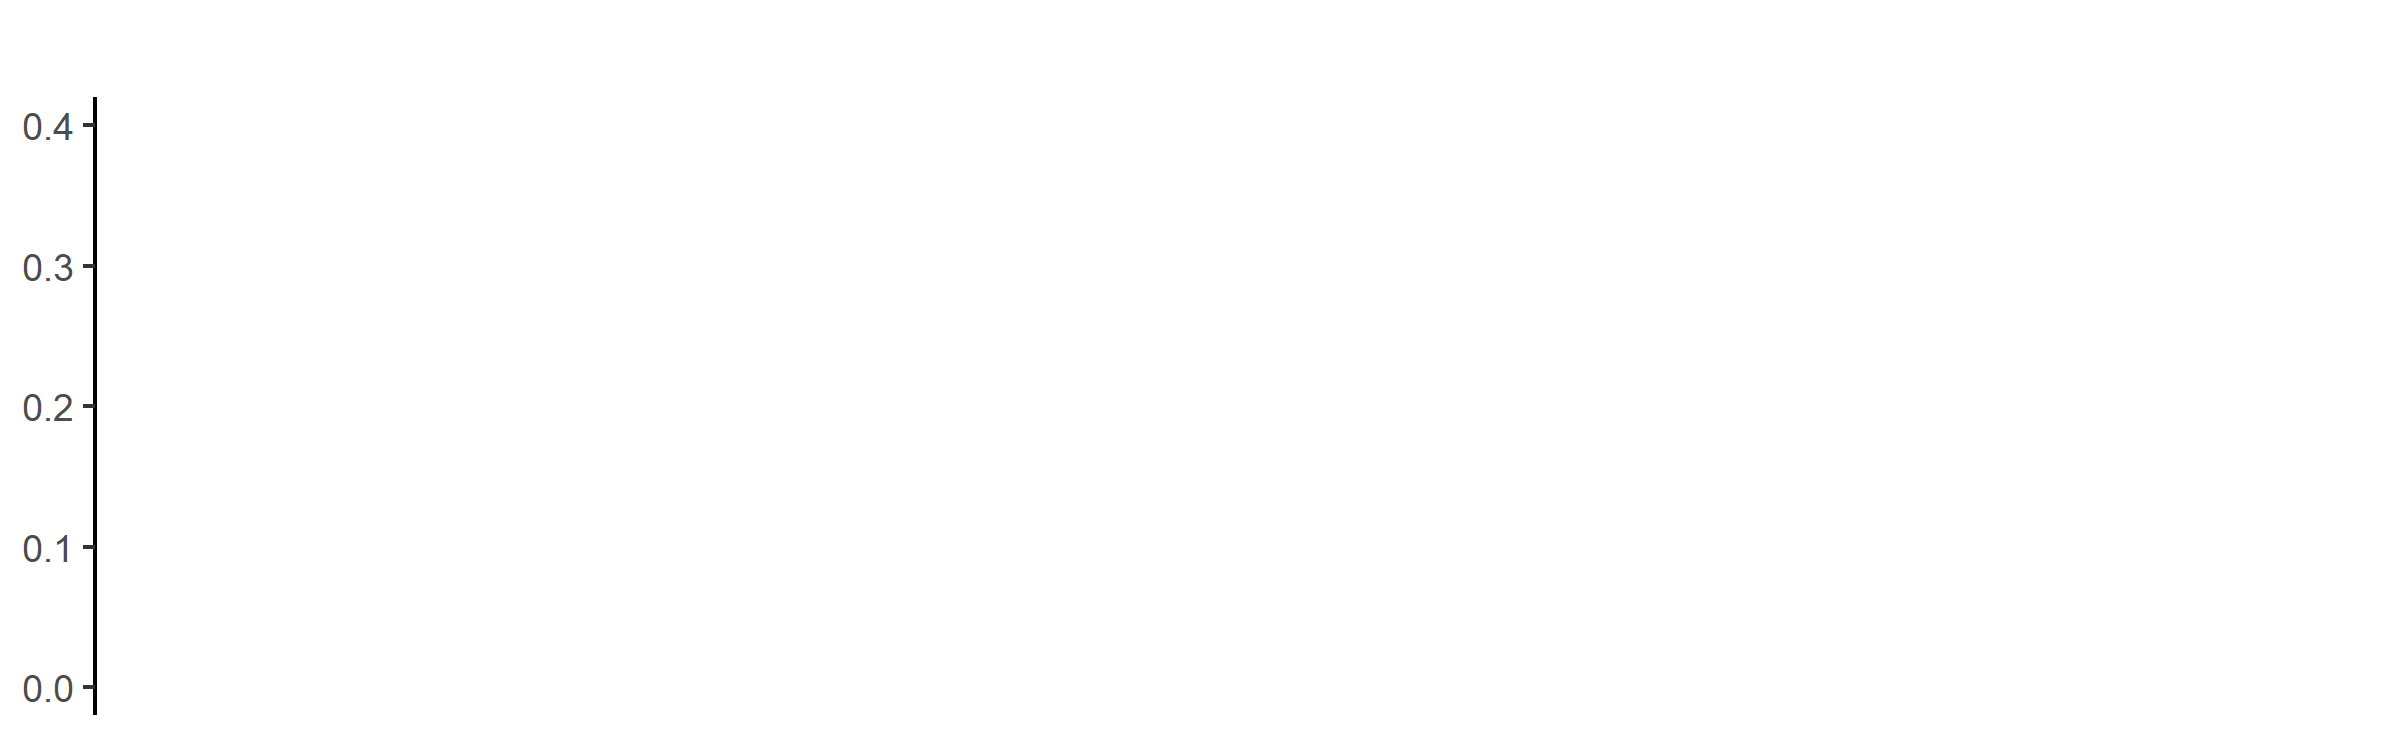
\includegraphics[width=\textwidth]{figure/200423_perturb_results_treat_add.png}
		\captionsetup{singlelinecheck=off, justification=centering}
		\caption{Adding Soc Trang back to treated group}
	\end{subfigure}
	\begin{subfigure}{.8\textwidth}
		\centering
		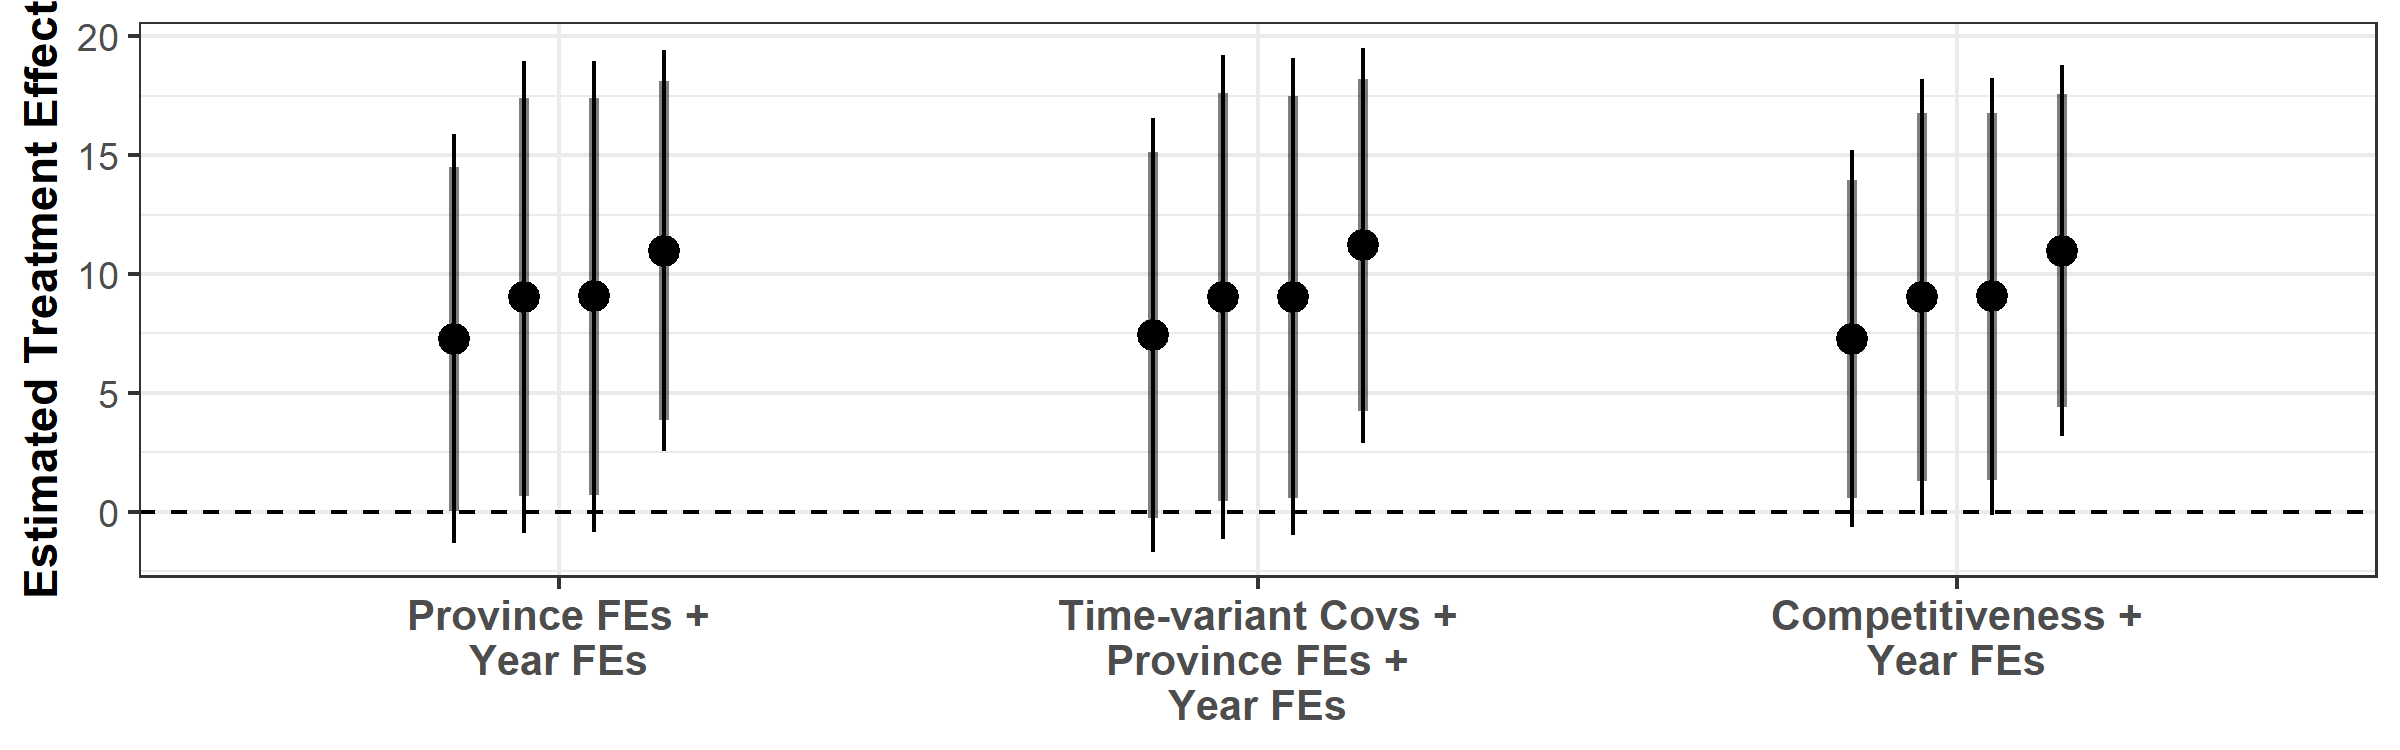
\includegraphics[width=\textwidth]{figure/200423_perturb_results_treat_drop.png}
		\captionsetup{singlelinecheck=off, justification=centering}
		\caption{Dropping one treated province}
	\end{subfigure}
	\begin{subfigure}{.8\textwidth}
		\centering
		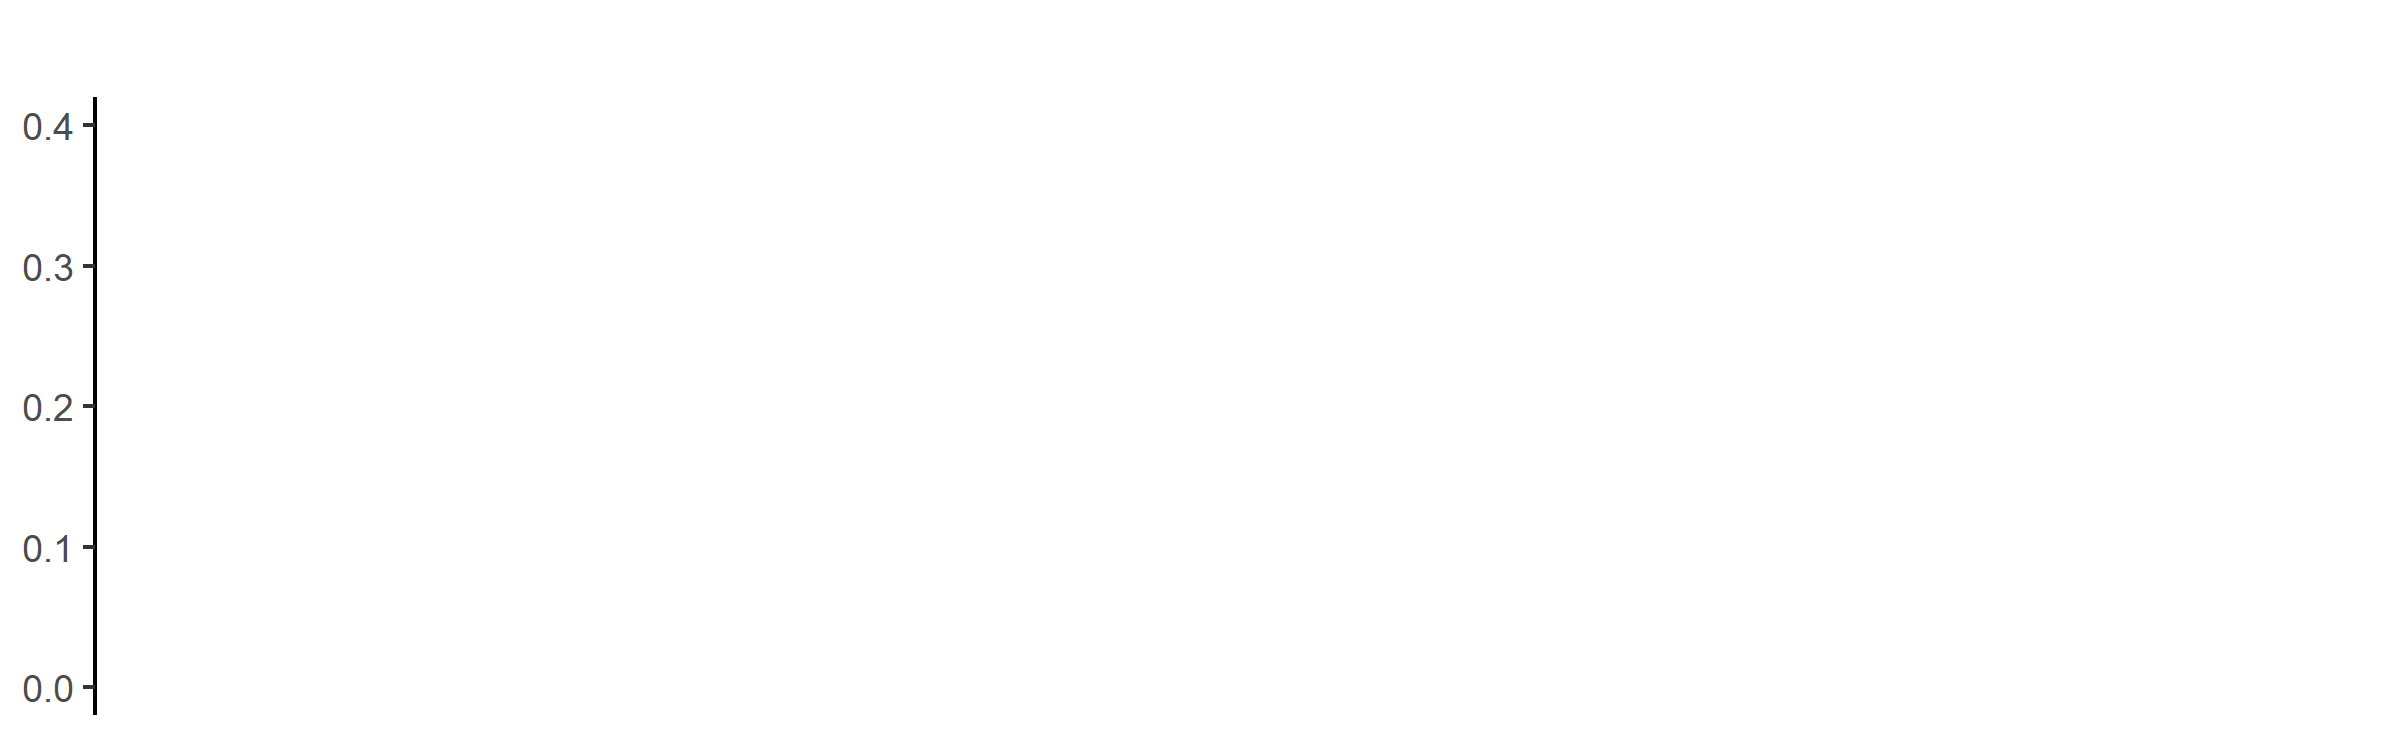
\includegraphics[width=\textwidth]{figure/200423_perturb_results_control_add.png}
		\captionsetup{singlelinecheck=off, justification=centering}
		\caption{Adding one control province}
	\end{subfigure}
	\begin{subfigure}{.8\textwidth}
		\centering
		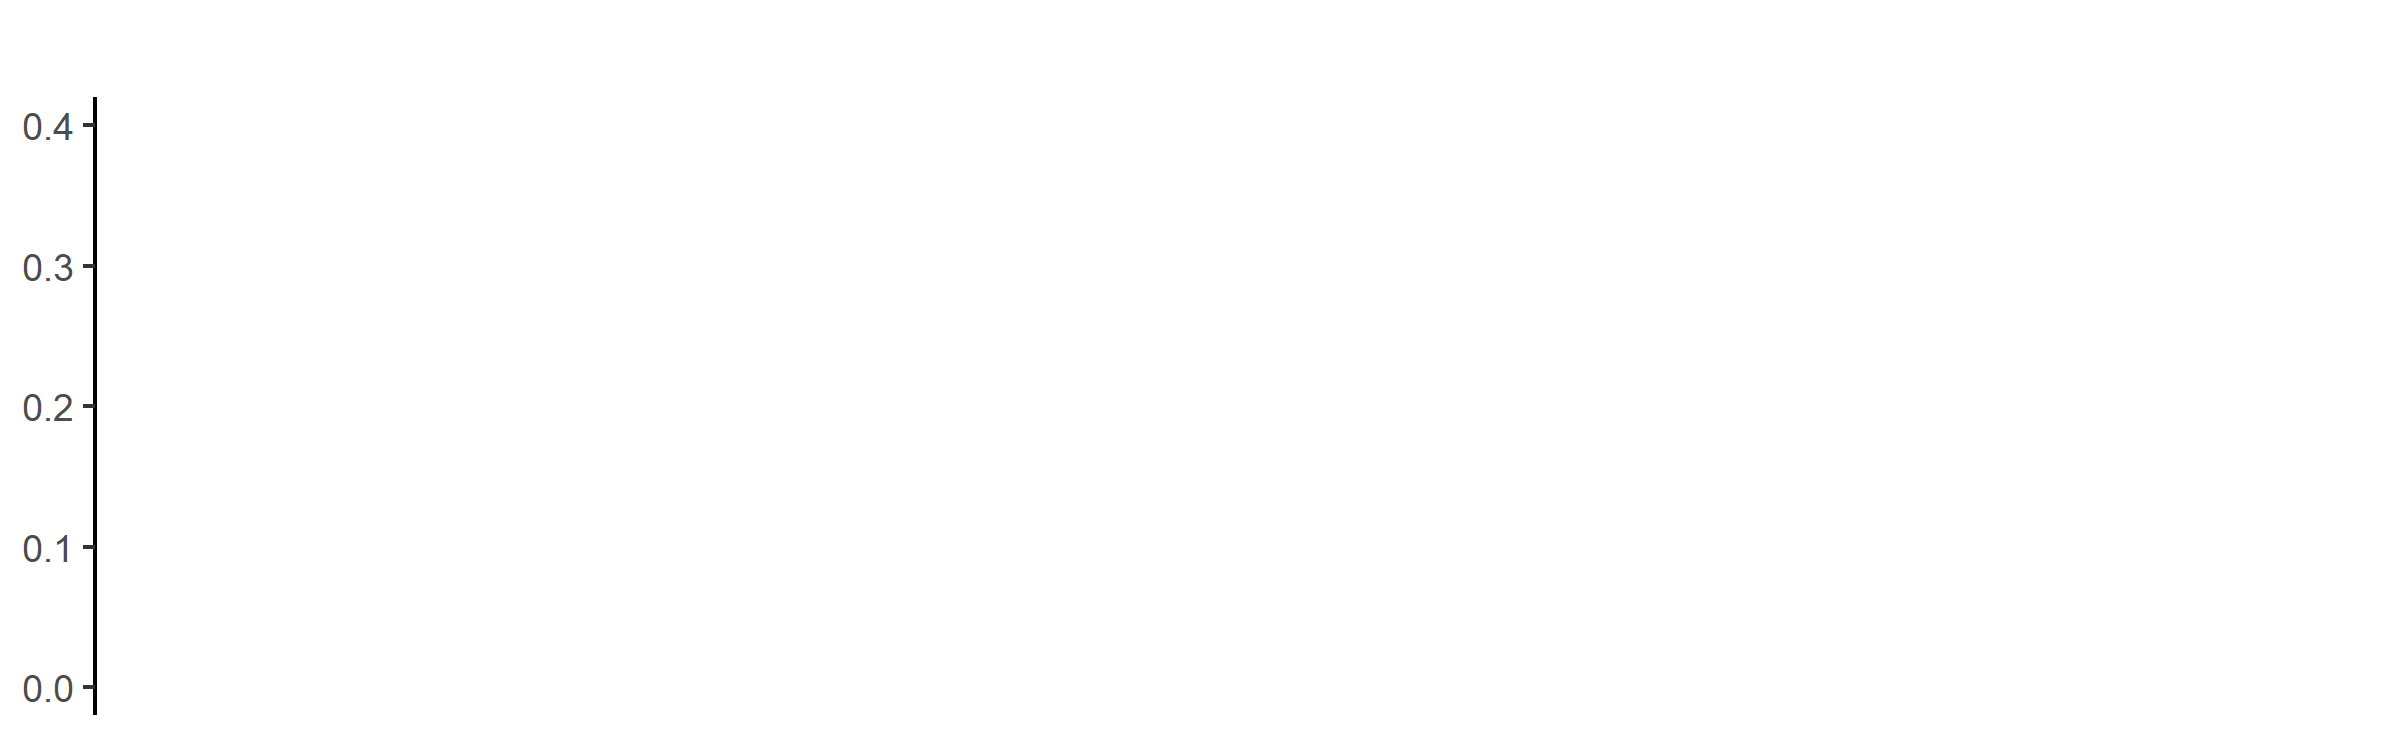
\includegraphics[width=\textwidth]{figure/200423_perturb_results_control_drop.png}
		\captionsetup{singlelinecheck=off, justification=centering}
		\caption{Dropping one control province}
	\end{subfigure}
	\caption[Estimated linear fixed effects treatment effects for perturbed samples]{Estimates of instantaneous treatment effects using linear fixed effects models on perturbed samples under different perturbation procedures. Thick error bars show 90\% confidence intervals and thin error bars show 95\% confidence intervals.}
	\label{fig:lfe_perturb}
\end{figure}

The distributions of instantaneous treatment effects estimated using the perturbed samples are plotted separately for each perturbation procedure in \autoref{fig:lfe_perturb}. In every plot, all the point estimates are close to each other -- and to the original estimates -- suggesting that they are not sensitive to perturbations to the sample. Although the procedure adds noise, nearly the estimates are found to be statistically significant, with the majority being significant at the .05 level and nearly all remaining estimates being significant at the .1 level. Even more reassuringly, all but a couple of  estimates for the persistent treatment effects (not shown here) are significant at the .05 level. This confirms that the main findings are unlikely to be artifacts of the specific sample and the specific composition of control and treated provinces in the data. 

\clearpage 
\section{Extending main analysis to previous elections}
\label{app:previous_elections}

\subsection{Why focus on the 2016 election?}

The analysis in the main manuscript focuses on the 2016 election to achieve the maximum inferential leverage. Compared to previous elections in 2011 and 2007\fnote{Data from elections before 2007 are not available.} the 2016 election offers significantly more valuable data in two ways. First, only in 2016 did the CPV include vote shares for defeated candidates when releasing election results. Official result releases in previous elections would only list out the names and vote shares of elected candidates, along with district-level statistics such as turnout. Although it is possible to identify defeated candidates can still be identified by comparing the pre-election candidate list with the final results, it is impossible to determine the margin by which each of them has lost. 

Information about margins is important because it helps separate out central candidate defeats that were close and hence truly informative from defeats that seemed too certain to contain new information. Central candidates who lost by large margins are likely to be different from those who did only narrowly, and provinces where heavy defeats happened are also likely to be different as well. At the candidate level, heavy losers may be unpopular with both the voting public and the provincial Party apparatus. Although unlikely, they may also be ``undesirable'' elites that the ruling party wishes to punish by forcing to contest an unwinnable election. At the province level, heavy defeats are more likely to signal blatant acts of resistance by provincial officials, acts that could only be expected from the most defiant provinces, which are also likely to be those most financially independent of the central government. In each of these scenarios, what sets the candidates or the provinces apart -- the candidates' unpopularity or the provinces' defiance -- must be serious enough that it cannot go unnoticed. In other words, when heavy defeats happen, the central leadership is likely to already know the underlying causes. Unlike close defeats which may have surprised the CPV, heavy defeats thus bring less information content, and are less likely to elicit the same kind of response. Including these defeats in the analysis would lead to no new insights about how the regime acquires and reacts to new information from elections, and in practice may lead to biased estimates.

Specifically, bias induced by the uniqueness of heavy defeats could manifest in two different ways. Firstly, if these defeats were not surprising and thus did not induce any reaction by the regime, then an estimate of their ``treatment effect'' would likely be zero, which would then bias the average treatment effect estimate downwards. Conversely, if heavy defeats actually indicated successful attempts by provincial officials to punish undesirable elites on behalf of the regime, then estimates of the average treatment effect would be inflated by any budgetary rewards that the provinces may receive for such successes. Secondly and more importantly, if heavy defeats reflected high degree of independence by the provinces, then both the level of central transfers these provinces received in the election year, as well as the year-to-year changes over preceding years, would likely be different. The result is the problem of dynamic causality \parencite{ImaiKim2019}, occurring because past central transfers are almost certainly determinants of present central candidate defeats. Because provinces with heavy defeats differ from provinces with no defeats both in the level of potential outcomes as well as the probability of receiving defeats, the difference in post-election central transfers between these sets of provinces no longer reflects a true, unbiased treatment effect of localized defeats. In other words, even if the central government also adjusted central transfers to these provinces in response to the heavy defeats, an estimate based on these provinces would still be biased by other confounders unrelated to the treatment of interest. 

Thus, the selection strategy using close victories and defeats is necessary because it ensures that the estimated changes in central transfers are attributed to information from the defeats alone. For 2016, only one central candidate defeat was heavy enough to be excluded under this selection strategy, but there is no guarantee that heavy central candidate defeats had been similarly rare in 2011 and 2007. On the contrary, as my analysis later in this section will show, that attempts to separate heavy defeats from close ones using information on vote shares yield large variations in treatment effect estimates, suggesting that confounding is serious for these two past elections.

Additionally, margins are also necessary in determining the close wins that would form the control group. Even though vote shares for central candidates who won are known, the margins by which they won cannot be determined without the vote share of the defeated candidates immediately behind them in the race. Because the vote shares of defeated candidates vary and may even exceed 50\%, using thresholds based on winners' vote shares alone may easily lead to false negatives. 

In the 2016 election, 7 out of 15 close central candidate victories were won with winners' vote shares above 60\%, such that using this threshold to identify close wins would have caused 5 provinces to wrongly drop out of the control set. This would have resulted in a loss in precision.

The second benefit of focusing on the 2016 election is that it offers a longer pre-treatment period for the generalized synthetic control method \citep{Xu2017gsynth}. Given that budgetary data for Vietnam is only available from 2004, an analysis focused on the 2016 election and hence designating 2017 as the first post-treatment year would have 13 pre-treatment years, much closer to \citepos{Abadie2010} recommendation than the 8 pre-treatment years available for an analysis focused on the 2011 election. The longer pre-treatment period allows more data to go into the construction of the synthetic control, which in turn leads to a more inferentially valid comparison. In addition, the synthetic control constructed from thinner data is less likely to perfectly match treated observations' outcome history, and is thus less effective at tackling dynamic causality.

When the sample is dynamically balanced like in the main analysis i.e. when treated and control provinces have similar outcome values in multiple pre-treatment years, inferences using the generalized synthetic control method are unlikely to diverge from linear fixed effects models, and thus function primarily to further validate these results. When there is significant threat of dynamic causality, however, the generalized synthetic control method is the only way to mitigate this problem. Because the sample from the 2007 and 2011 elections are likely to suffer from dynamic causality, but does not have sufficient data for the generalized synthetic control method to perform optimally, the main analysis prioritizes data from the 2016 election to achieve the maximum level of internal validity.

\subsection{Responses to localized defeats in 2011 election}

Even though focusing on the 2016 election would lead to the most internally valid inferences, external validity requires that I identify whether similar increases in central transfers can also be observed following localized defeats of central candidates in previous elections. I thus attempt to extend the main analysis in this paper to the 2011 and 2007 elections, the only remaining elections for which data is available, starting with the 2011 election.

As discussed above, I anticipate several analytical challenges. For the linear fixed effects models, the lack of data on margins means that analyses will be restricted to the ``naive'' sample that count all provinces with any central candidate defeat as treated and all provinces with central candidate winning with less than 60 percent vote share as control. In other words, I am likely to over-count treated provinces and under-count control provinces. This is expected to result in important pre-treatment dissimilarity between treated and control provinces as well as weaker precision. Although the models' inferences are only valid for provinces with narrow central candidate victories and defeats, the 2011 treated pool also contains an unknown number of provinces with only heavy defeats. Because these provinces are not comparable to provinces with close central candidate defeats, and thus are not comparable to provinces with close central candidate victories, estimates of the treatment effect is likely to be biased. \autoref{fig:lfe_placebo_2011}, which plots estimates of the treatment effect using the ``naive'' sample for the 2011 election, against three placebo treatment effects estimated by assuming the 2011 election has instead happened in 2008, 2009, and 2010, confirms this concern. Specifically, there are large placebo effects detected for 2009 and 2010, which should not be expected if treated and control provinces are comparable. The placebo instantaneous effects for 2009 in particular are large in magnitude and, depending on specification, are statistically significant at either the .1 or .05 level (although not shown here, all placebo persistent effects for 2009 are significant at the .05 level). When compared to placebo effects estimated in the 2016 analysis, each placebo effect for 2011 is larger than the corresponding effect for 2016, suggesting serious dynamic imbalance with the ``naive'' sample. For this reason, the main effect estimates, which are negative and indistinguishable from zero, should not be considered as reliable.

\begin{figure}[!htbp]
	\centering
	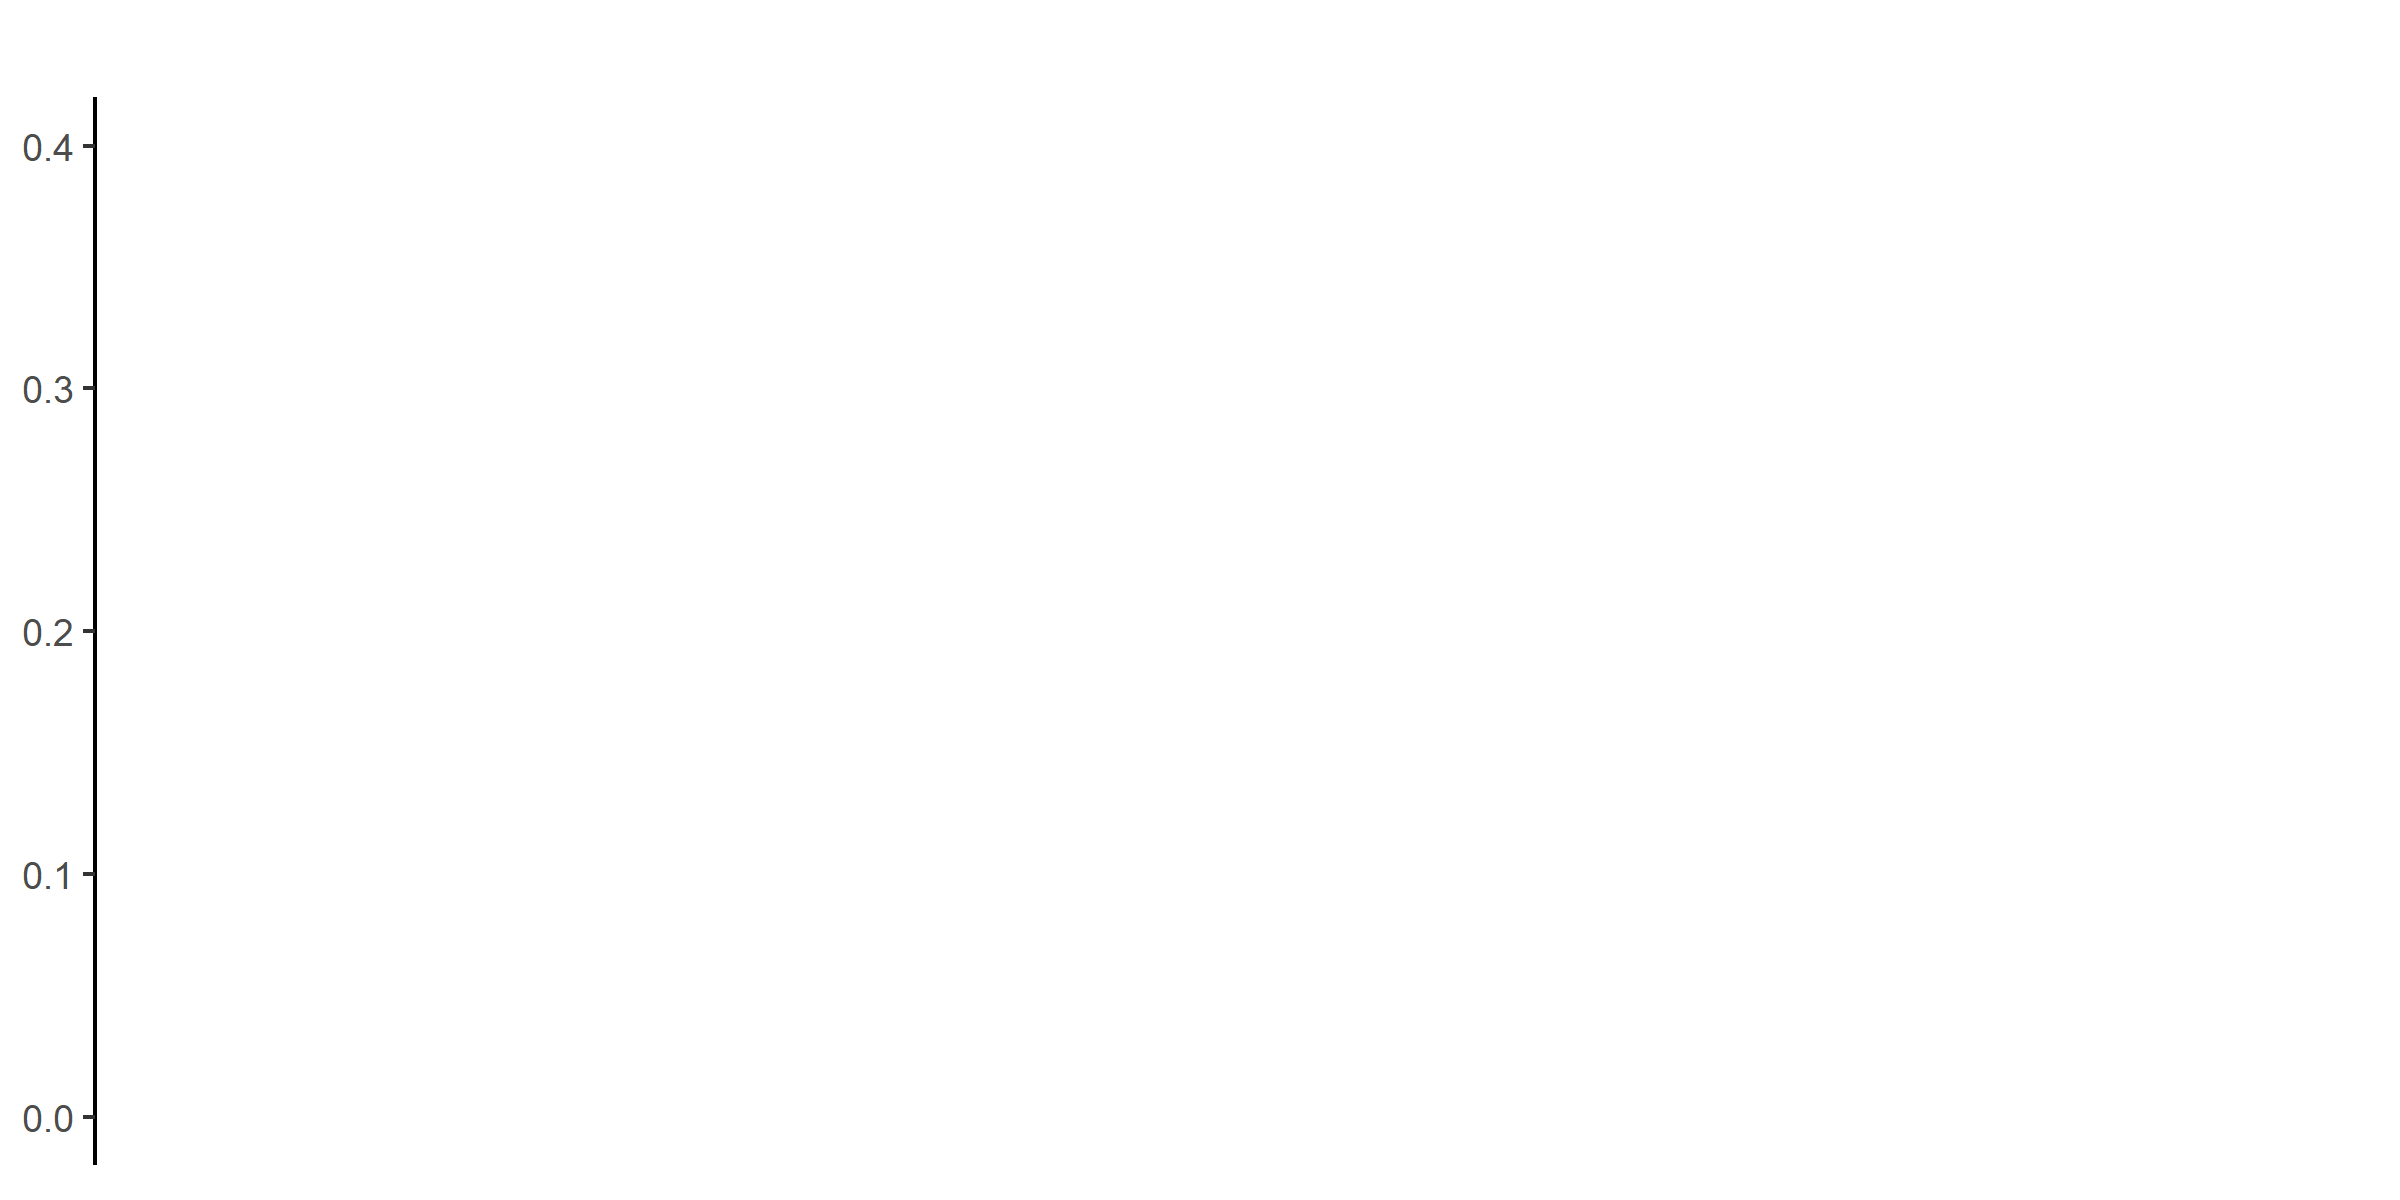
\includegraphics[width=\textwidth]{figure/200422_lfe_placebo_2011.png}
	\captionsetup{singlelinecheck=off}
	\caption[Estimated placebo linear fixed effects treatment effects for 2011]{Estimates of persistent treatment effects for the 2011 election using linear fixed effects models. All central candidate defeats are included in the sample. The error bars show 95\% confidence intervals.}
	\label{fig:lfe_placebo_2011}
\end{figure}

To compound the problem, the candidate-level local randomization procedure is no longer appropriate for this case. Recall that this procedure involves identifying a window of vote margin boundaries, such that central candidates who lost and won with margins within this window can be considered to have had their result assigned as-if randomly. Without vote share data from defeated candidates to calculate margins, no such boundaries can be defined. The closest alternative is an one-sided window defined by an upper boundary on winners' vote shares, such that the sample would include all central candidates who won with vote shares smaller than it. The resulting window, however, would still include all defeated central candidates, including those whose defeats are too severe to ever be considered as-if random. This undermines the logic of the regression discontinuity framework, and thus would not lead to appropriate inferences.

In light of the problem facing the linear fixed effects analysis, and the inapplicability of the local randomization approach, the generalized synthetic control method \citep{Xu2017gsynth} becomes much more important. Compared to linear fixed effects model, it is more effective at addressing dynamic causality, even when it is unable to account for unobserved time-invariant confounders \autocite{ImaiKim2019}. Given the possibility of dynamic imbalance revealed in \autoref{fig:lfe_placebo_2011}, this method seems preferable for the 2011 analysis.

\autoref{fig:synth_results_2011} shows the result from an analysis applying the generalized synthetic control method \citep{Xu2017gsynth} to data from the 2011 election. Most importantly, it shows that estimates of localized defeats' treatment effect is positive in all post-treatment years, with magnitude increasing the further away from the election year and becoming statistically significant (at the .05 level) in 2015. The method has mitigated pre-treatment differences in net transfers between treated and control provinces, as evident in the much smaller placebo treatment effects at 2009, 2010, and 2011. Because it uses data from only a short pre-treatment period, however, the generalized synthetic control in this analysis is still far from a perfect match to the treated pool. In particular, some concerns about dynamic imbalance remain, given that the difference in outcome at 2011 is still statistically significant at the .1 level. At the same time, when compared with results from the linear fixed effects, it is possible to see that the magnitude of the treatment effect increases as dynamic imbalance is reduced, suggesting that the confounding induced by dynamic causality may have led to a downward bias. In any case, the evidence from this analysis, though tentative, does suggest a positive effect i.e. an increase in central transfers to provinces that experienced localized defeats.

\begin{figure}[!h]
	\centering
	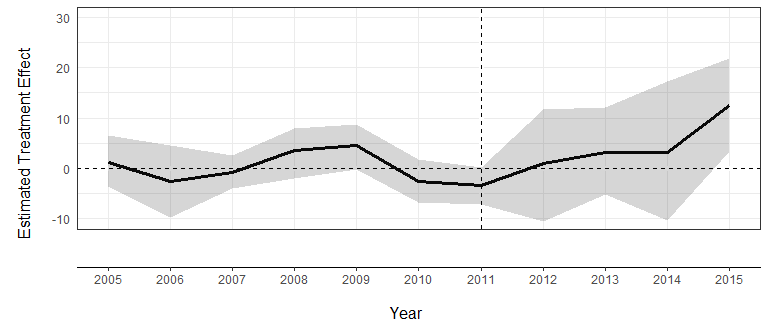
\includegraphics[width=\textwidth]{figure/200202_synth_results_2011.png}
	\captionsetup{singlelinecheck=off}
	\caption[Estimated synthetic control treatment effects for 2011]{Estimates of treatment effects for the 2011 election using the generalized synthetic control method. All central candidate defeats are included in the sample. The horizontal dashed line marks the election year.}
	\label{fig:synth_results_2011}
\end{figure}

To confirm that the positive treatment effect identified by the generalized synthetic control method \citep{Xu2017gsynth} is indeed appropriate and not the result of unprincipled cherry-picking, I show that this result is achievable with linear fixed effects models if cases of close victories and defeats could be identified. To do this, I use available data on winning candidates' vote shares to simulate a large number of educated guesses about defeated candidates' performance, construct indicators of central candidates' close victories and defeats based on these guesses, and then estimate plausible treatment effects based on these indicators. The distribution of estimates obtained from this exercise will then cover the ``true'' treatment effects that would have been identified when all data is available.

Educated guesses about defeated candidates' vote shares are possible because these shares are not completely unknowable. Because Vietnam's electoral rules specify that each voter gets to vote for as many candidates as there are seats in the district, the maximum value of the sum of all candidates' vote shares in the districts is 100 percent times the number of seats. For example, in a district with five candidates and three seats, the sum of all five candidates' vote shares must not exceed 300 percent. For each district, the sum of all the losers' vote shares must not exceed the difference between this maximum sum and the sum of all the winners' vote shares -- data for which is available. In addition, each individual loser's vote share cannot exceed that of the lowest winning candidate (or, in districts with unfilled seats, the 50 percent threshold). Altogether, these facts limit the range within which each defeated candidate's vote share could lie.

Given the above limit, I simulate possible values for all the defeated central candidates by randomly allocating the ``left-over'' vote shares that did not belong to the winning candidates in each districts among the losers, leaving aside also a small share representing unallocated votes from voters who did not use up all their votes or those who voted for write-in candidates. Specifically, for each district with $k$ defeated candidates, I draw random samples of proportions from the constrained $(k+1)$-simplex, with the constraints defined by the maximum vote share a defeated candidate could secure as well as an upper limit of .1 on the share of unallocated votes, and distribute the ``left-over'' vote shares according to these proportions.\fnote{The constraint on unallocated vote shares is based on the expectation that votes rarely go unallocated and on the observed distribution of these votes in the 2016 election}\fnote{A probability simplex is a vector of probability $p_1, p_2, \dots, p_k$ such that $\sum_{k}^{i=1}p_i = 1$. Random samples from the simplex is done with random draws from the Dirichlet distribution. To avoid making assumptions about the relative distribution of vote shares among defeated candidates, I draw from the uniform Dirichlet distribution with $\mathbf{\alpha} = \mathbf{1}$, and enforce the constraints with rejection sampling. A more efficient sampling method is to draw from a distribution with $\alpha_i > 1$, but this assumes that highly unequal distribution of votes among defeated candidates are unlikely. Yet another method is to model the shape parameters for each district based on observed data for 2016, which requires additional modeling assumptions. In practice, different sampling approaches yield very similar results.} With a large number of draws, the resulting distribution will approximate the universe of all possible values of the unobserved vote shares.

Then, taking each random allocation of vote shares as one hypothetical observation of the defeated candidates' vote shares, I calculate winning and losing margins for all central candidates, and use these margins to construct district-level and province-level indicators of localized defeats. The resulting distribution of province-level treatment indicator vectors from this step provides the unconditional likelihood that each province has experienced close central candidate victories or narrow localized defeats. Intuitively, in provinces where winning local candidates have secured a large number of votes, it is difficult for the losing central candidates to have also won enough votes to remain in close proximity to the lowest winning winner, especially if they also had to split votes with the other losers. In these provinces the size of the ``left-over'' vote shares is small, and few random allocations of this already small pool among losing candidates can result in one having enough to remain within a 10 percentage point of the winners.

Using the province-level treatment indicator vectors from the previous step, I fit the linear fixed effects models in the main analysis to estimate a set of treatment effects corresponding to each vector. Each model may use a different sample depending on the randomly drawn vote shares, but provinces where central candidates are only likely to lose with large margins will be excluded more frequently. The distribution of estimates from this exercise represents the universe of possible treatment effects that could have been estimated from the universe of feasible vote share allocations, and thus takes into account the likelihood that each defeat or victory could be truly close. The true values of the treatment effects i.e. what could have been estimated had real data on vote shares are available, has to fall within it. This distribution does not serve an inferential purpose, as the true estimate is a fixed value and exists independent of the simulated vote shares. In addition, it assigns equal likelihood for every feasible allocations of vote shares within a district, even though the reality on the ground could be much more complicated. At the same time, in the absence of additional information, it offers the most reliable and assumption-free guidance on which values of the treatment effects are more likely.

\begin{figure}[!htbp]
	\centering
	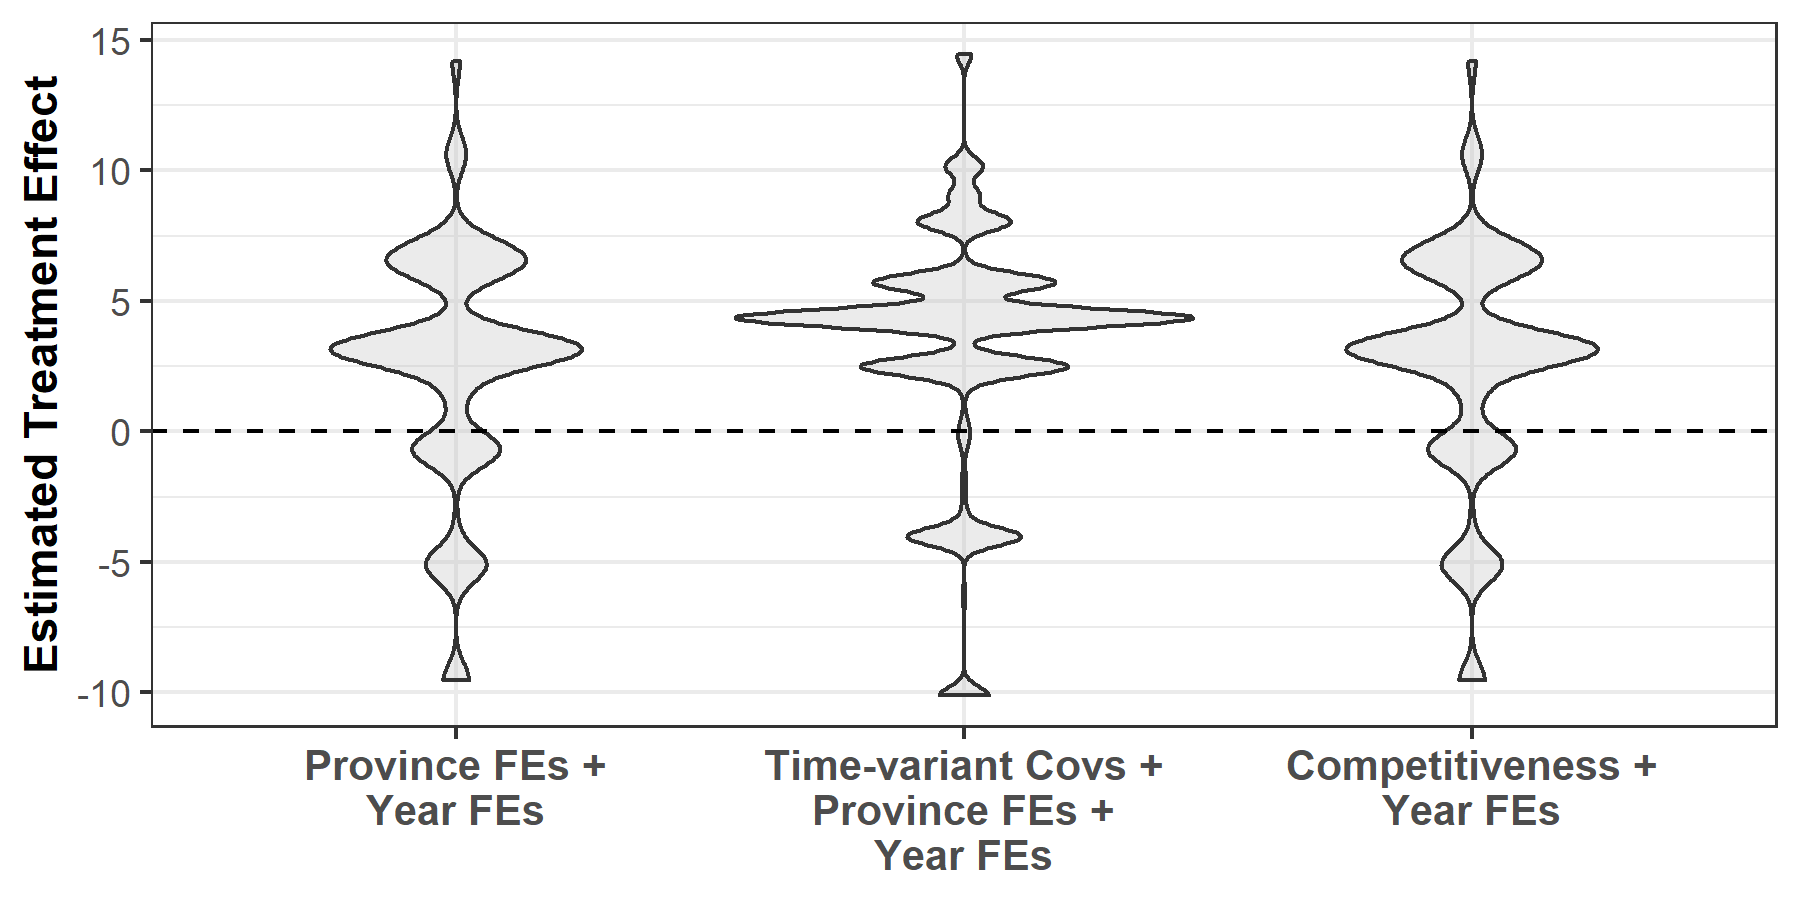
\includegraphics[width=.75\textwidth]{figure/200423_impute_results_2011.png}
	\captionsetup{singlelinecheck=off}
	\caption[Estimated linear fixed effects treatment effects using simulated vote shares]{Distribution of estimates of persistent treatment effects using linear fixed effects models on simulated samples. Each sample may include a different set of central candidate defeats and victories.}
	\label{fig:impute_results_2011}
\end{figure}

Distributions of estimated treatment effects using all the linear fixed effects models in the main analysis, obtained from $10000$ independent simulations of the vote shares, are shown in \autoref{fig:impute_results_2011}. It shows that the majority of the estimates are positive. Depending on specification, between .72 to .85 of the estimates are larger than zero. In other words, for the true estimate of localized defeats' treatment effects to be negative, the true vote shares of defeated candidates must have taken values that are highly improbable given the winning candidates' performance. Additionally, the negative estimates in \autoref{fig:lfe_placebo_2011} are close to the minimum values from the distributions, suggesting that almost any feasible allocations of defeated candidates' vote shares would lead to higher treatment effects. Altogether, although this evidence does not eliminate the possibility that the true treatment effect may be negative or close to zero, it does confirm that the linear fixed effects analysis using the entire sample of defeated central candidates is likely to be inaccurate. The generalized synthetic control method \citep{Xu2017gsynth}, on the other hand, not only addresses some concern about dynamic causality, but also produces estimates that seem much more probable. 

Overall, the positive effect from this analysis suggests that the CPV also reacted to localized defeats of its central candidates in the 2011 election by increasing central transfers to provinces that experienced such defeats. This finding, although much more tentative, is consistent with the result for the 2016 election.
 
\subsection{Responses to localized defeats in 2007 election}

The analysis for the 2007 election faces even more severe problems than the 2011 analysis. \autoref{fig:lfe_placebo_2007} shows estimates of the treatment effects, along with two sets of placebo treatment effects estimated for 2005 and 2006 (no placebo analysis is done for 2004 due to insufficient data). All these estimates are based on a sample with the entire set of central candidate defeats. The main treatment effects are estimated to be positive but not statistically significant, but the large and statistically significant (at .1 level, for some specifications) placebo treatment effects suggest that these estimates are likely to be inaccurate.

\begin{figure}[!htbp]
	\centering
	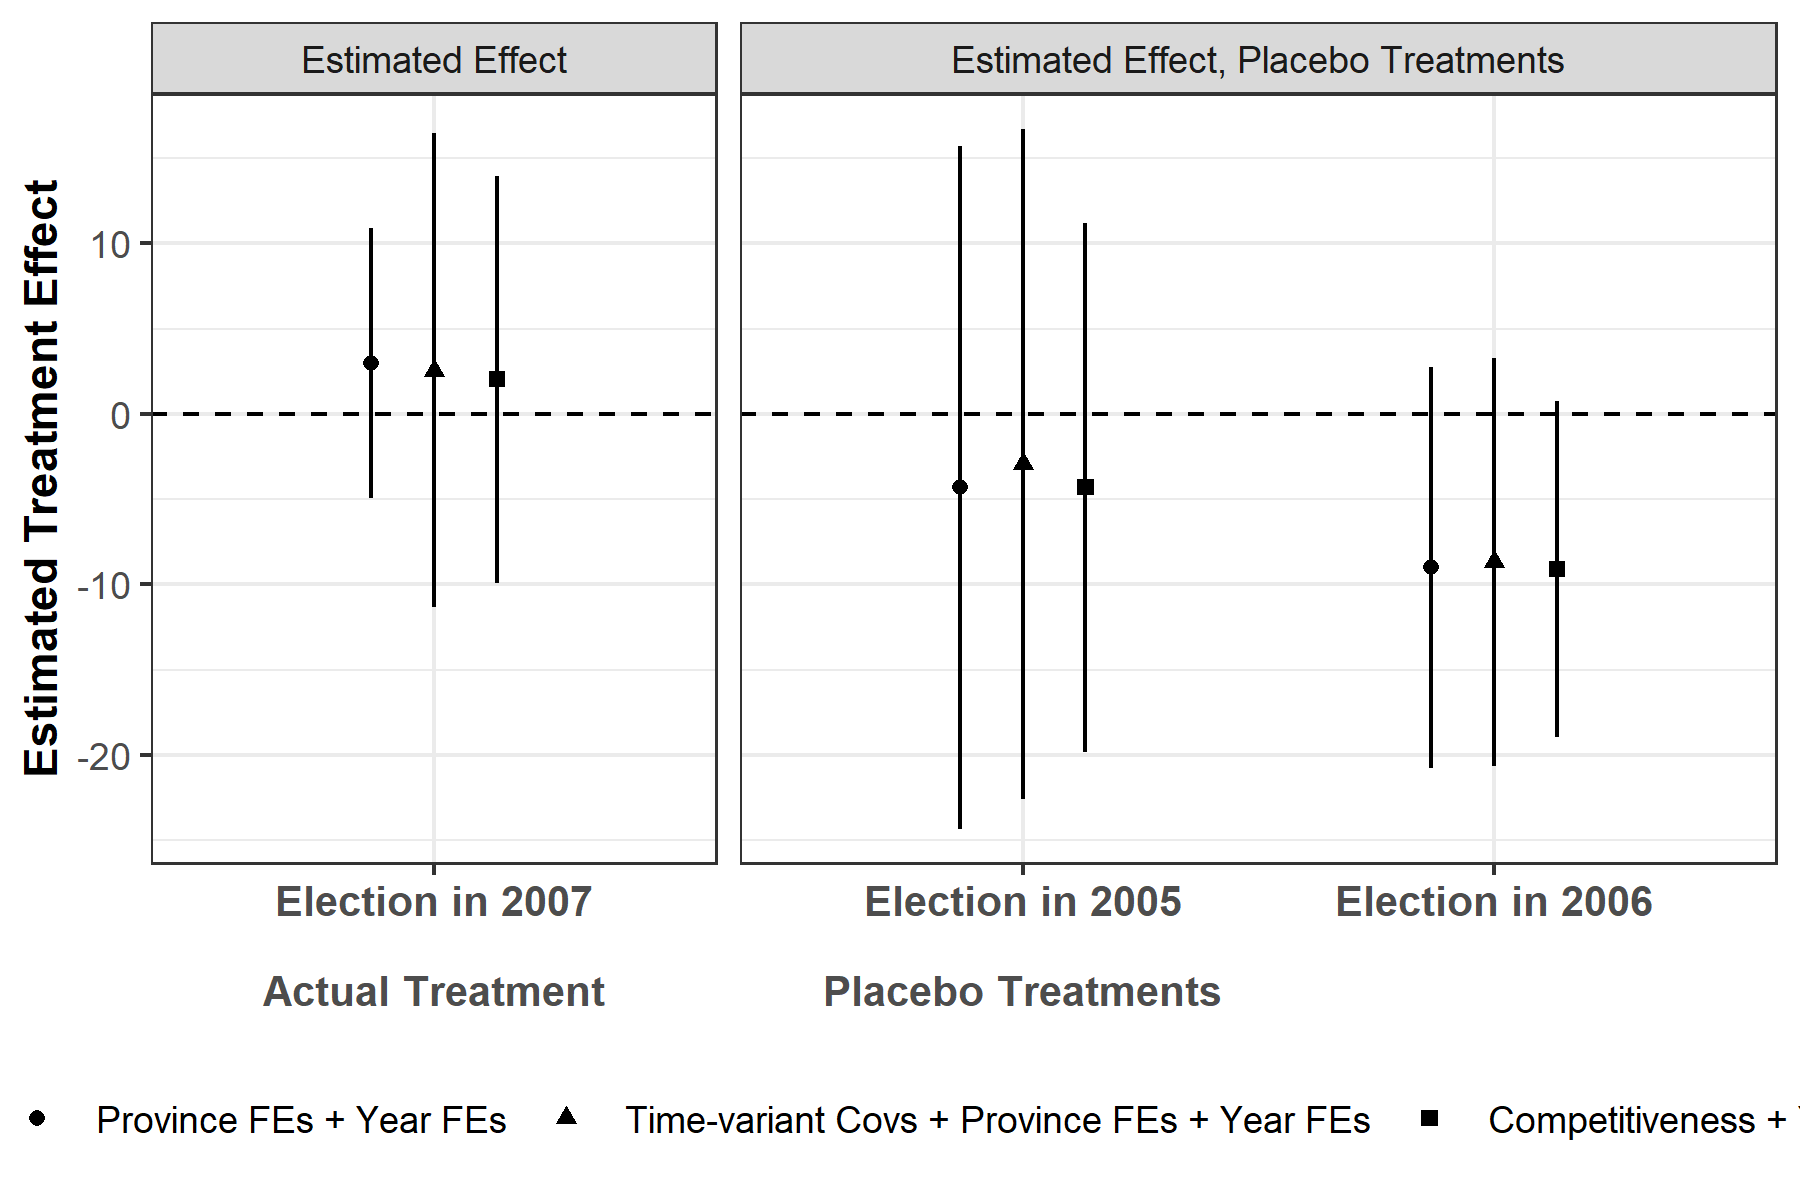
\includegraphics[width=.75\textwidth]{figure/200202_lfe_placebo_2007.png}
	\captionsetup{singlelinecheck=off}
	\caption[Estimated placebo linear fixed effects treatment effects]{Estimates of instantaneous treatment effects using linear fixed effects models. All central candidate defeats are included in the sample. The error bars show 95\% confidence intervals.}
	\label{fig:lfe_placebo_2007}
\end{figure}

Unlike in the 2011 analysis, the generalized synthetic control method \citep{Xu2017gsynth} is not applicable for 2007 data because there are too few pre-treatment years to construct reliable synthetic controls. There is thus no reliable means to mitigate or eliminate the threat of dynamic causality evident in the large placebo effects. 

\begin{figure}[!htbp]
	\centering
	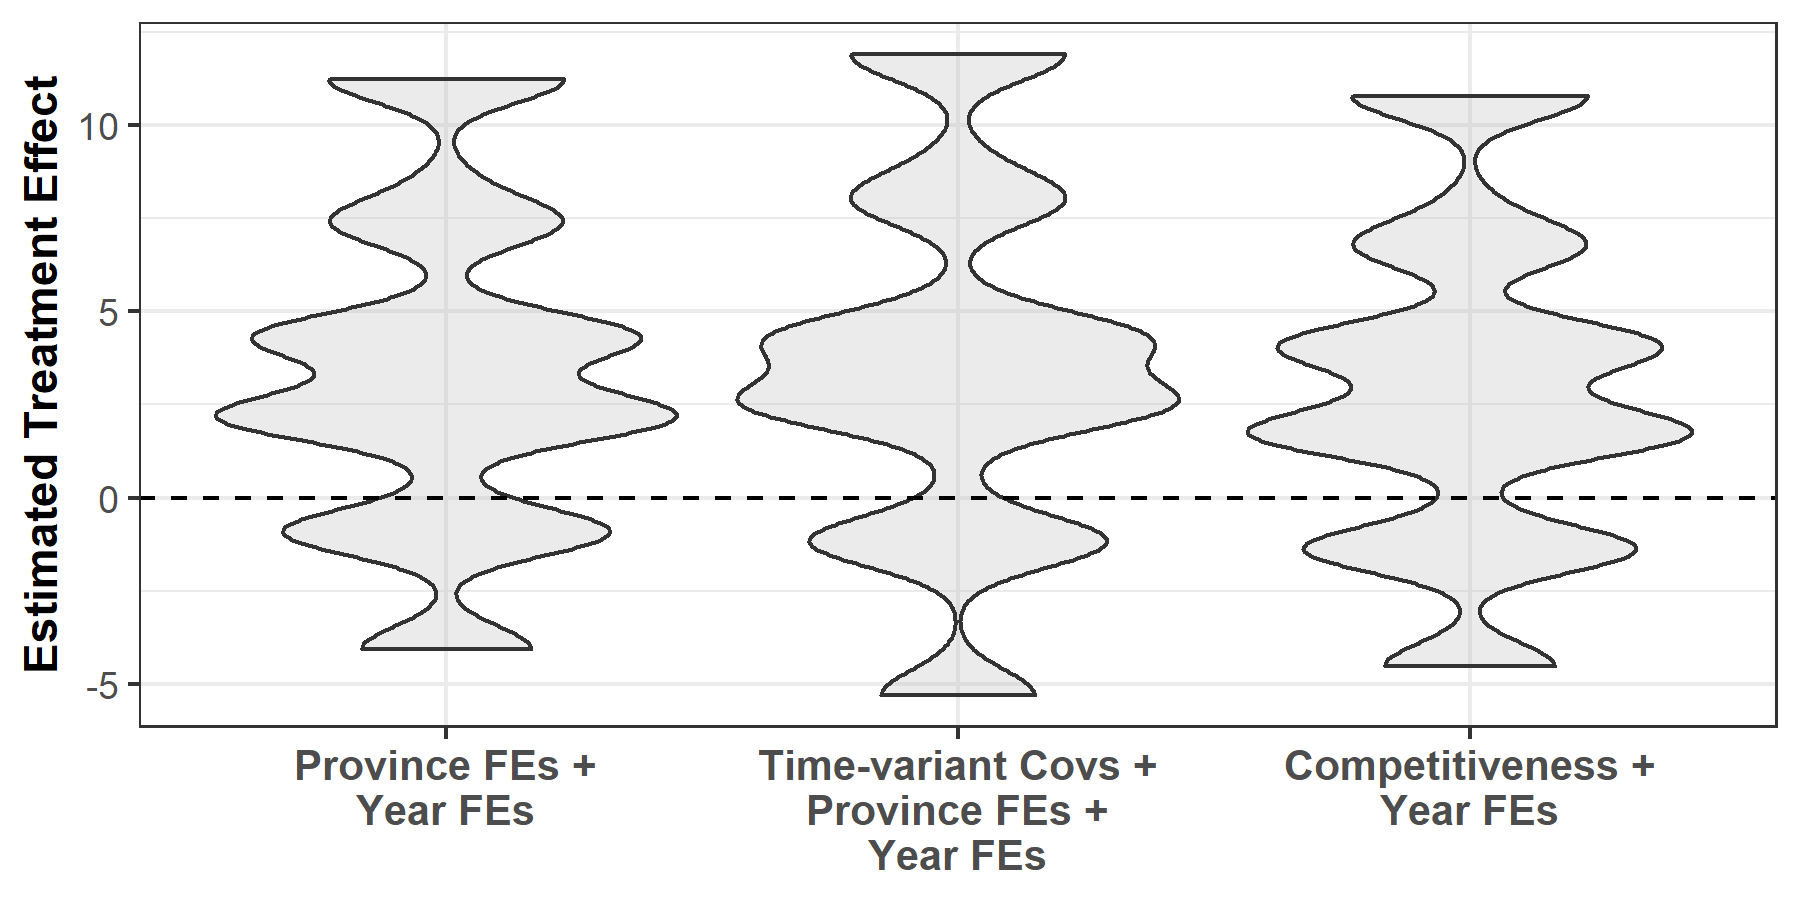
\includegraphics[width=.75\textwidth]{figure/200202_impute_results_2007.png}
	\captionsetup{singlelinecheck=off}
	\caption[Estimated linear fixed effects treatment effects using simulated vote shares]{Distribution of estimates of instantaneous treatment effects using linear fixed effects models on simulated samples. Each sample may include a different set of central candidate defeats and victories.}
	\label{fig:impute_results_2007}
\end{figure}

However, by simulating feasible vote shares of defeated candidates, I still find that the true estimates for the effect of localized defeats on central transfers, obtained when cases of heavy and unsurprising defeats have been excluded, are more likely to be positive. Specifically, \autoref{fig:impute_results_2007}, which shows the distribution of treatment effect estimates obtained from $10000$ simulations of vote shares for the defeatd candidates, confirms that the majority of feasible treatment effects are positive. Similar to the 2011 results, both the mean and median of the estimates are positive, with around .74 of the estimates found to be larger than zero. Even though much more data is needed for a stronger conclusion, this evidence does offer some reason to believe that the true treatment effects are larger than what found by the ``naive'' linear fixed effects models. Indeed, they are much more likely to be positive, which is consistent with the results for both the 2011 and 2016 elections.

\clearpage

\section{Causal mechanism: effects on development and administrative spending}
\label{app:mechanisms}

In Section \ref{sec:additional} of the main manuscript, I argue that a narrative in which the CPV increased central transfers to provinces it suffered defeats in to placate dissatisfied voters must be accompanied by evidence of an increase in development spending and an absence of cuts in administrative spending in these districts. Table \ref{tab:lfe_mech} and Figure \ref{fig:synth_rdd_mech} present this evidence, with the former presenting estimates from linear fixed effects model and the latter showing graphically the results from the local randomization regression discontinuity and generalized synthetic control analyses. There are positive and stable treatment effects on both outcomes, but the effect on development spending is bigger even though it only approaches statistical significance. Compared to the analyses in Section \ref{sec:methods_estimation}, the only difference is that the linear fixed effects models in this section do not use log-differenced outcome. This is because detailed budget breakdowns are available only for a subset of provinces, and then are sporadically missing for some years. Calculating log-differences would only exacerbate this missingness. This caveat changes the interpretation of the treatment effect's magnitude but does not compromise its validity, as every specification still passes all placebo tests.


% Table created by stargazer v.5.2.2 by Marek Hlavac, Harvard University. E-mail: hlavac at fas.harvard.edu
% Date and time: Wed, Feb 19, 2020 - 3:23:26 AM
\begin{table}[!htbp] \centering 
  \caption{Estimated treatment effects of localized defeats on development and administration expenditures from linear fixed effects models} 
  \label{tab:lfe_mech} 
\begin{tabular}{@{\extracolsep{5pt}}lcccccc} 
\\[-1.8ex]\hline 
\hline \\[-1.8ex] 
 & \multicolumn{3}{c}{Development Expenditure} & \multicolumn{3}{c}{Administrative Expenditure} \\ 
\\[-1.8ex] & (1) & (2) & (3) & (4) & (5) & (6)\\ 
\hline \\[-1.8ex] 
 Treatment Effect & 0.406 & 0.440 & 0.392 & 0.265 & 0.283 & 0.260 \\ 
  & (0.298) & (0.283) & (0.274) & (0.198) & (0.206) & (0.182) \\ 
 \hline \\[-1.8ex] 
Election Competitiveness &  &  & Yes &  &  & Yes \\ 
Time-invariant Covariates &  & Yes &  &  & Yes &  \\ 
Province FEs & Yes & Yes &  & Yes & Yes &  \\ 
Year FEs & Yes & Yes & Yes & Yes & Yes & Yes \\ 
\hline \\[-1.8ex] 
N & 68 & 68 & 68 & 68 & 68 & 68 \\ 
R$^{2}$ & 0.834 & 0.849 & 0.531 & 0.657 & 0.675 & 0.449 \\ 
\hline 
\hline \\[-1.8ex] 
\multicolumn{7}{l}{$^{*}$p $<$ .1; $^{**}$p $<$ .05; $^{***}$p $<$ .01} \\ 
\end{tabular} 
\end{table} 


\begin{figure}[!htbp]
	\centering
	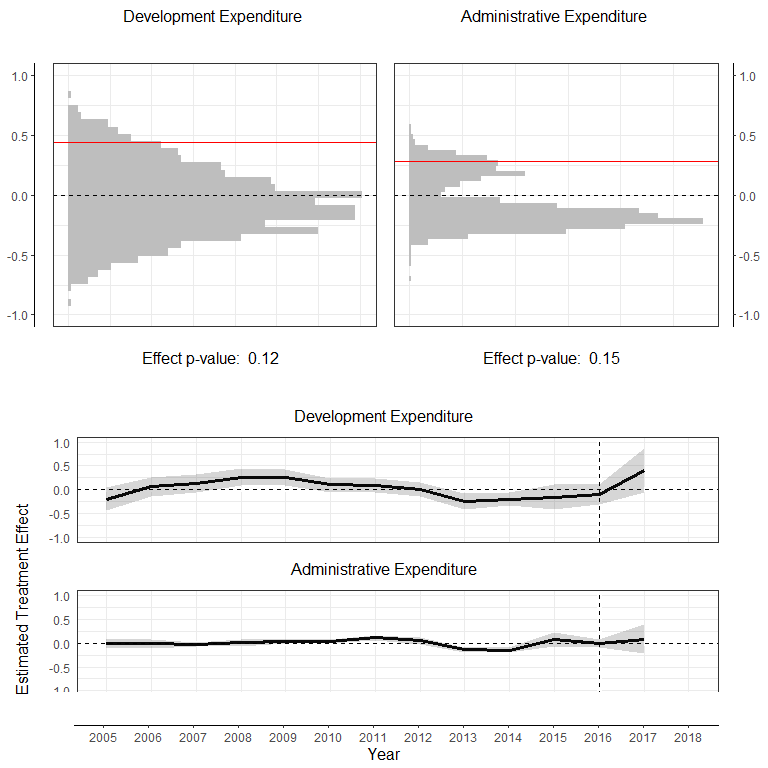
\includegraphics[width=\textwidth]{figure/200205_mech_results.png}
	\captionsetup{singlelinecheck=off}
	\caption[Estimated RDD and synthetic control treatment effects]{Estimates of treatment effects on development and administrative expenditure using RDD under the local randomization approach and the generalized synthetic control method. Only effects for 2017 are calculated due to lack of 2018 data.}
	\label{fig:synth_rdd_mech}
\end{figure}

\clearpage

\section{Individual treatment effect for Can Tho}
\label{app:alt_mech}

In Can Tho's second electoral district, the 2016 election saw four candidates competed for two seats in the VNA. Among them, Nguyen Van Quyen, a 63-year-old native of Ninh Binh, is the central candidate. He is the Party Secretary and Chairman of the Vietnam Lawyers Association -- a state-sanctioned organization of legal professionals operating in parallel with the Vietnam Bar Association. Outside of his role in the Lawyers Association, Nguyen Van Quyen also serves in the central leadership of Vietnam Fatherland Front (VFF) -- the umbrella institution with which all mass organizations must be affiliated -- and in a 16-delegate committee on judicial reforms within the CPV central leadership. His multiple roles as leader of a central-level mass organization and a high-ranking CPV official earn him a nomination by the central leadership. Following several \textit{hiệp thương} rounds, he was sent to run in the second district of Can Tho, a province that he has had no experience in.

Also competing in this district are three local candidates: Tran Quoc Trung, the sitting Party Secretary of Can Tho and member of the CPV Central Committee; Ngo Trung Quan, a local business owner who also holds a rank-and-file position in the VFF Central Committee; and Dao Thi Sa Ron, a vice-principal of a local public school. 

\begin{table}[htb]
	\caption{Candidate profiles and election results, Can Tho's second electoral district}
	\label{tab:cantho_mech}
	\resizebox{\textwidth}{!}{%
		\begin{tabular}[t]{@{}llllll@{}}
			\\[-1.8ex] 
			\hline
			\hline
			\\[-1.8ex]
			Name & Age & Gender & Nominator & Professional Profile  & Vote Share (\%) \\ \midrule
			Tran Quoc Trung & 56  & Male   & Local & \begin{tabular}[c]{@{}l@{}}Can Tho Party Secretary\\ Member, \\ \hspace{10pt} CPV Central Committee\end{tabular} & 74.35  \\ \\[-1.8ex] \hline \\[-1.8ex]
			Ngo Trung Quan  & 56  & Male   & Local & \begin{tabular}[c]{@{}l@{}}Member, \\ \hspace{10pt} VFF Central Committee\\ Local Business Owner\end{tabular}    & 49.09   \\ \\[-1.8ex] \hline \\[-1.8ex]
			\textbf{Nguyen Van Quyen} & 63 & Male & Central & \begin{tabular}[c]{@{}l@{}} Chairman, \\ \hspace{10pt} Vietnam Lawyers Association\\ Deputy Party Secretary and Vice Chairman, \\ \hspace{10pt} VFF Central Committee\\ Member, \\ \hspace{10pt} CPV Committee on Judicial Reforms\end{tabular} & 47.12 \\ \\[-1.8ex] \hline \\[-1.8ex]
			Dao Thi Sa Ron  & 43  & Female & Local & \begin{tabular}[c]{@{}l@{}} Vice Principal, \\ \hspace{10pt} Can Tho Boarding School for \\ \hspace{10pt} Ethnic Minorities \end{tabular} & 28.24 \\
		    \\[-1.8ex] 
			\hline
			\hline
			\\[-1.8ex]
		\end{tabular}%
	}
\end{table}

With two seats up for contest, it would have been possible for both the central candidate Nguyen Van Quyen and the provincial chief Tran Quoc Trung to both win. With each voter casting two votes, the total vote shares among all four candidates in this election is 200\%. However, because Tran Quoc Trung ended up securing a large number of votes -- 74.35\% -- the remaining vote shares were split thinly among all three remaining candidates, as seen in Table \ref{tab:cantho_mech}. As a result, none of them secured approval from more than 50\% of the voters, thus failing to pass the minimum threshold for election. Nguyen Van Quyen himself was supported by 47.12\% of the voters.

The large vote shares given to the strong local candidate Tran Quoc Trung thus play an important role in the central candidate defeat in Can Tho. The CPV could interpret this as either as a result of Tran Quoc Trung exerting too much effort to get himself elected, or of Can Tho voters' disapproval of the central regime. An increase in central transfers to Can Tho would show that the CPV believes in the latter interpretation. Yet, another hypothesis suggests that increases in transfers to provinces with defeated central candidates could have resulted from these provinces having more local candidates elected and thus a greater voice in the budget allocation process. However, in the case of Can Tho, because no local candidate captured the empty seat,\fnote{In a second election round in which three defeated candidates competed for the empty seats, Nguyen Van Quyen won with 55.11\% of votes and ended up taking this seat.} this election result did not lead to an increased representation for the province in the VNA. An increase in central transfers to Can Tho therefore could not have been triggered by VNA representation. Observing this effect still manifesting would thus rule out the alternative hypothesis.

\begin{figure}[!h]
	\centering
	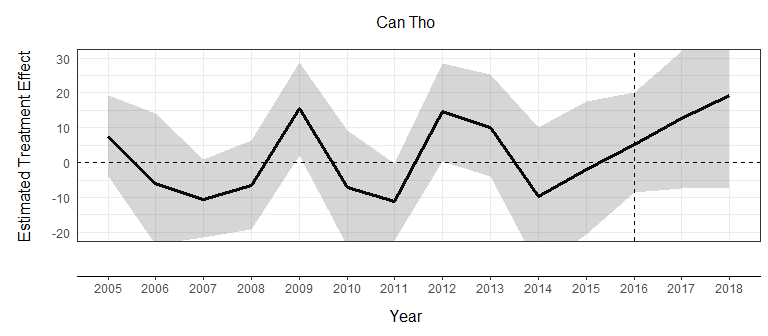
\includegraphics[width=\textwidth]{figure/200205_synth_results_CanTho.png}
	\captionsetup{singlelinecheck=off}
	\caption[Individual synthetic control treatment effect]{Individual estimate of treatment effects on central transfers for Can Tho, estimated using the generalized synthetic control method similar to \autoref{fig:synth_placebo}.}
	\label{fig:synth_mech}
\end{figure}

Because the generalized synthetic control method allows treatment effects to be extracted for individual units, I show in Figure \ref{fig:synth_mech} that Can Tho did indeed experience increased central transfers in 2017 and 2018 when compared to the synthetic control. Although the 95\% confidence intervals are large and cross zero due to insufficient power, the point estimates suggest that it saw large a large increase in central transfers of approximately 20\% of previous years' annual change; this is also the largest year-to-year increase ever observed in Can Tho since data becomes available. While this finding is far from conclusive, it does offer some good evidence to dismiss negotiation and bargaining through representation as the primary driver for the main treatment effects.

\clearpage
\section{Absence of other punishment for leaders in provinces with central defeats, 2007 and 2011}
\label{app:punishment}

To further confirm that provincial leaders did not receive punishment for central candidate defeats, I use data on the career tracks of top Vietnamese politicians provided by \citet{MaleskyPhan2017} to see whether these defeats have had any impact on their career prospects. The data allows me to identify for all officials who have ever governed in a province -- defined as holding one of the top two provincial leadership positions -- whether they have gone on to hold higher positions in the Party or government hierarchies. I conduct this test only on officials who were governing before the 2007 and 2011 elections however, because those governing in 2016 would not have completed their current term. Thus, the test would provide evidence only on whether the CPV has historically had a tendency to punish provincial officials for central career defeats

The data in Table \ref{tab:promo_mech} shows the number of provinces that have had zero, one, or both of its top leaders promoted, separated by treatment status. In case there is shuffling of provincial leadership in the election year, I calculated promotion records for both leaders who are in power \textit{before} and \textit{during} the election year. This would account for both the possibilities that the CPV sees elections as a referendum on either the governing performance or the election management performance of provincial officials. I count promotion events over the entire term i.e. 2006-2010 for those governing in 2005 and 2006, and 2011-2015 for those governing in 2010 and 2011.

% latex table generated in R 3.6.0 by xtable 1.8-4 package
% Fri Apr 24 01:15:07 2020
\begin{table}[ht]
\centering
\begin{tabular}{lcccccccc}
   & \multicolumn{2}{c}{Gov. in 2006} & \multicolumn{2}{c}{Gov. in 2007} & \multicolumn{2}{c}{Gov. in 2010} & \multicolumn{2}{c}{Gov. in 2011} \\
 & $T = 0$ & $T = 1$ & $T = 0$ & $T = 1$ & $T = 0$ & $T = 1$ & $T = 0$ & $T = 1$ \\
 \hline
No Promotion & 1 & 3 & 1 & 3 & 3 & 4 & 2 & 3 \\ 
  1 Promotion & 5 & 2 & 5 & 2 & 3 & 2 & 4 & 2 \\ 
  2 Promotions & 0 & 0 & 0 & 0 & 2 & 1 & 2 & 2 \\ 
   \hline
Fisher Odd Ratio & 0.16 &  & 0.16 &  & 0.48 &  & 0.47 &  \\ 
  Fisher p-value & 0.20 &  & 0.20 &  & 0.40 &  & 0.43 &  \\ 
  \end{tabular}
\caption{Summary of promotion records for the top two leaders in all the provinces in the restricted sample. 
             Promotion records are calculated for leaders who are in power in 2006 (ruling just before the 2007 election), 2007 (in charge of managing the 2007 election),
             2010 (ruling just before the 2011 election), and 2011 (in charge of managing the 2011 election).} 
\label{tab:promo_mech}
\end{table}


Table \ref{tab:promo_mech} shows no significant difference in the frequency of promotion among officials in provinces with and without central candidate defeats. Where there seems to be a difference, the gap is never big enough for a Fisher's exact test to reject the null hypothesis. This evidence suggests that the top party leadership did not delay the promotion of provincial officials even when central candidate defeats had happened under their jurisdiction.

This finding is consistent with the observation that, unlike in other nondemocratic regimes such as Russia \citep{Myagkov2009}, Vietnam's leaders rely on punishment much more sparingly, reserving demotion or firing only to very serious transgressions.\fnote{Two illustrative anecdotes suggest that the CPV avoids punishment because it draws attention to disunity within the party, and that it only punishes top officials in case of extreme transgressions. In 2012, when the CPV's highest leadership debated and decided against officially censuring then-PM Nguyen Tan Dung for economic mismanagement, official statements from the Party refers to him only as ``one comrade'' without mentioning any name \citep{voa2012}. Later, in 2017, when the Party's leaders finally decided to punish Ho Chi Minh City's Party Secretary Dinh La Thang and to publicly acknowledge this decision, it was only after mismanagement of PetroVietnam, Vietnam's largest SOE and where Thang had served as chairman between 2009 and 2001, has been found to cost the country close to US\$150 million \citep{BBC2017}.} In addition, the CPV only makes major personnel decisions at its Party Congress, which takes place every five year and usually just before an election (presumably so that the election could ratify and legitimize newly appointed leaders). This makes the time lag between one election's outcomes and the next batch of promotion decisions too large for the latter to be useful as punishment for the former.

%\section{Difference in central candidate vote shares as alternative measure}
%\label{app:share_dif}
%
%In theory, the CPV could detect surprisingly poor results by monitoring changes in central candidates' performances across elections. Specifically, they may be able to identify areas with poor regime supports by looking at provinces where the average central candidate secured much fewer votes in 2016 than in 2011, instead of just relying on wins and losses alone. If this is the case, then the Vietnamese regime should be expected to increase central transfers to provinces that experienced a big negative swing in central candidate vote shares across the two elections.
%
%This conceptualization of surprisingly poor results, however, does not seem to match with the CPV's narratives about election results, which have paid much more attention to regime defeats \citep[][e.g]{vov2016, laodong2016}. Practically, vote shares, or vote share swings, may suffer from more noises, and overall offers a less clear-cut signal than defeats or wins.
%
%Moreover, vote share changes are less helpful in helping to distinguish whether Hanoi sees in negative results information about regime popularity or about regime agents. Whereas a defeat can send both types of signal, a large vote share swing unaccompanied by central candidate defeat may even speak to local officials' ability to secure victory for central candidates without sacrificing votes for local elites. An increase in central transfers to provinces with this kind of swing may still be consistent with a story in which Hanoi rewards local officials who can capably balance both local and central interests.
%
%For the empirical analysis in this paper, operationalizing poor election results with negative vote swings may lead to two measurement problems. First, because vote share changes are by definition a function of vote shares in the previous election, this measurement is automatically dependent of past election results. Because past election results are also likely to influence both the pre-treatment trajectory of central transfers as well as the likelihood that negative results will happen again, the result is dynamic dependency between past treatment, past outcome and present treatment. This is likely to complicate the analysis.
%
%Second, because vote shares for defeated candidates in 2011 are not available, a measure of election performance using vote swings would have to exclude those past vote shares that are expected to be the lowest. This would lead to non-classical measurement error that ultimately would bias the treatment effect estimates.
%
%Finally, when analyzing the effect of vote share swings, empirical models must account for the possibilities that only large enough swings should matter for the regime, and that negative swings and positive swings may send different signals. This requires the model to allow non-linear effects, which may lead to unwanted researcher degrees-of-freedom.
%
%For these various reasons, I refrain from using vote share swings in the main analysis, and instead focus on the effect of wins and losses. Accounting for vote share swings, however, does not weaken the main findings. Specifically, in \autoref{tab:lfe_share}, I fit two linear fixed effects models -- one using vote share swings and a quadratic transformation, and one that also include indicators of central candidate defeats -- and used both models to estimate the instantaneous and persistent effects of the included variables. To facilitate interpretation of the quadratic terms, \autoref{fig:lfe_share} plots for each model the estimated treatment effects of an one-percentage increase in the magnitude of a province's vote swing against the very magnitude of this swing. As discussed above, the measurement of average provincial vote share swings in all the models do not take into account central candidates who lost in the 2011 election for whom data is unavailable.
%
%
% Table created by stargazer v.5.2.2 by Marek Hlavac, Harvard University. E-mail: hlavac at fas.harvard.edu
% Date and time: Tue, Feb 25, 2020 - 11:02:29 PM
\begin{table}[!htbp] \centering 
  \caption{Estimated effects of vote share swings on central transfers from linear fixed effects models} 
  \label{tab:lfe_share} 
\begin{tabular}{@{\extracolsep{5pt}}lcccc} 
\\[-1.8ex]\hline 
\hline \\[-1.8ex] 
 & \multicolumn{2}{c}{Instantaneous Effect} & \multicolumn{2}{c}{Persistent Effect} \\ 
\\[-1.8ex] & (1) & (2) & (3) & (4)\\ 
\hline \\[-1.8ex] 
 Vote Share Dif. & $-$0.133 & $-$0.181 & $-$0.023 & $-$0.032 \\ 
  & (0.196) & (0.191) & (0.168) & (0.165) \\ 
  Vote Share Dif.\textsuperscript{2} & 0.013 & 0.005 & 0.028$^{*}$ & 0.027$^{*}$ \\ 
  & (0.013) & (0.015) & (0.015) & (0.015) \\ 
  Election Defeat &  & 6.920$^{**}$ &  & 2.590 \\ 
  &  & (2.806) &  & (2.352) \\ 
 \hline \\[-1.8ex] 
Province FEs & Yes & Yes & Yes & Yes \\ 
Year FEs & Yes & Yes & Yes & Yes \\ 
\hline \\[-1.8ex] 
N & 300 & 300 & 360 & 360 \\ 
R$^{2}$ & 0.489 & 0.491 & 0.431 & 0.431 \\ 
\hline 
\hline \\[-1.8ex] 
\multicolumn{5}{l}{$^{*}$p $<$ .1; $^{**}$p $<$ .05; $^{***}$p $<$ .01} \\ 
\end{tabular} 
\end{table} 

%
%As seen in all the plots, the effect estimates are generally indistinguishable from zero, confirming my concerns about the reliability of the measure. It should still be noted, however, that the estimated effect does increase and become positive for larger values of vote swings, affirming the intuition that poor results may trigger regime response if they are large enough. Furthermore, including the defeat indicator in Models 3 and 5 dampens this effect, suggesting that large vote share swings and actual defeats are eliciting similar reactions from the CPV. Overall, this analysis shows that changes in vote share are not clear-cut enough to serve as a good operationalization and measurement of surprising setbacks, but also that the relationship between these changes and central transfers conform to the paper's primary evidence. 
%
%\begin{figure}[!hbp]
%	\centering
%	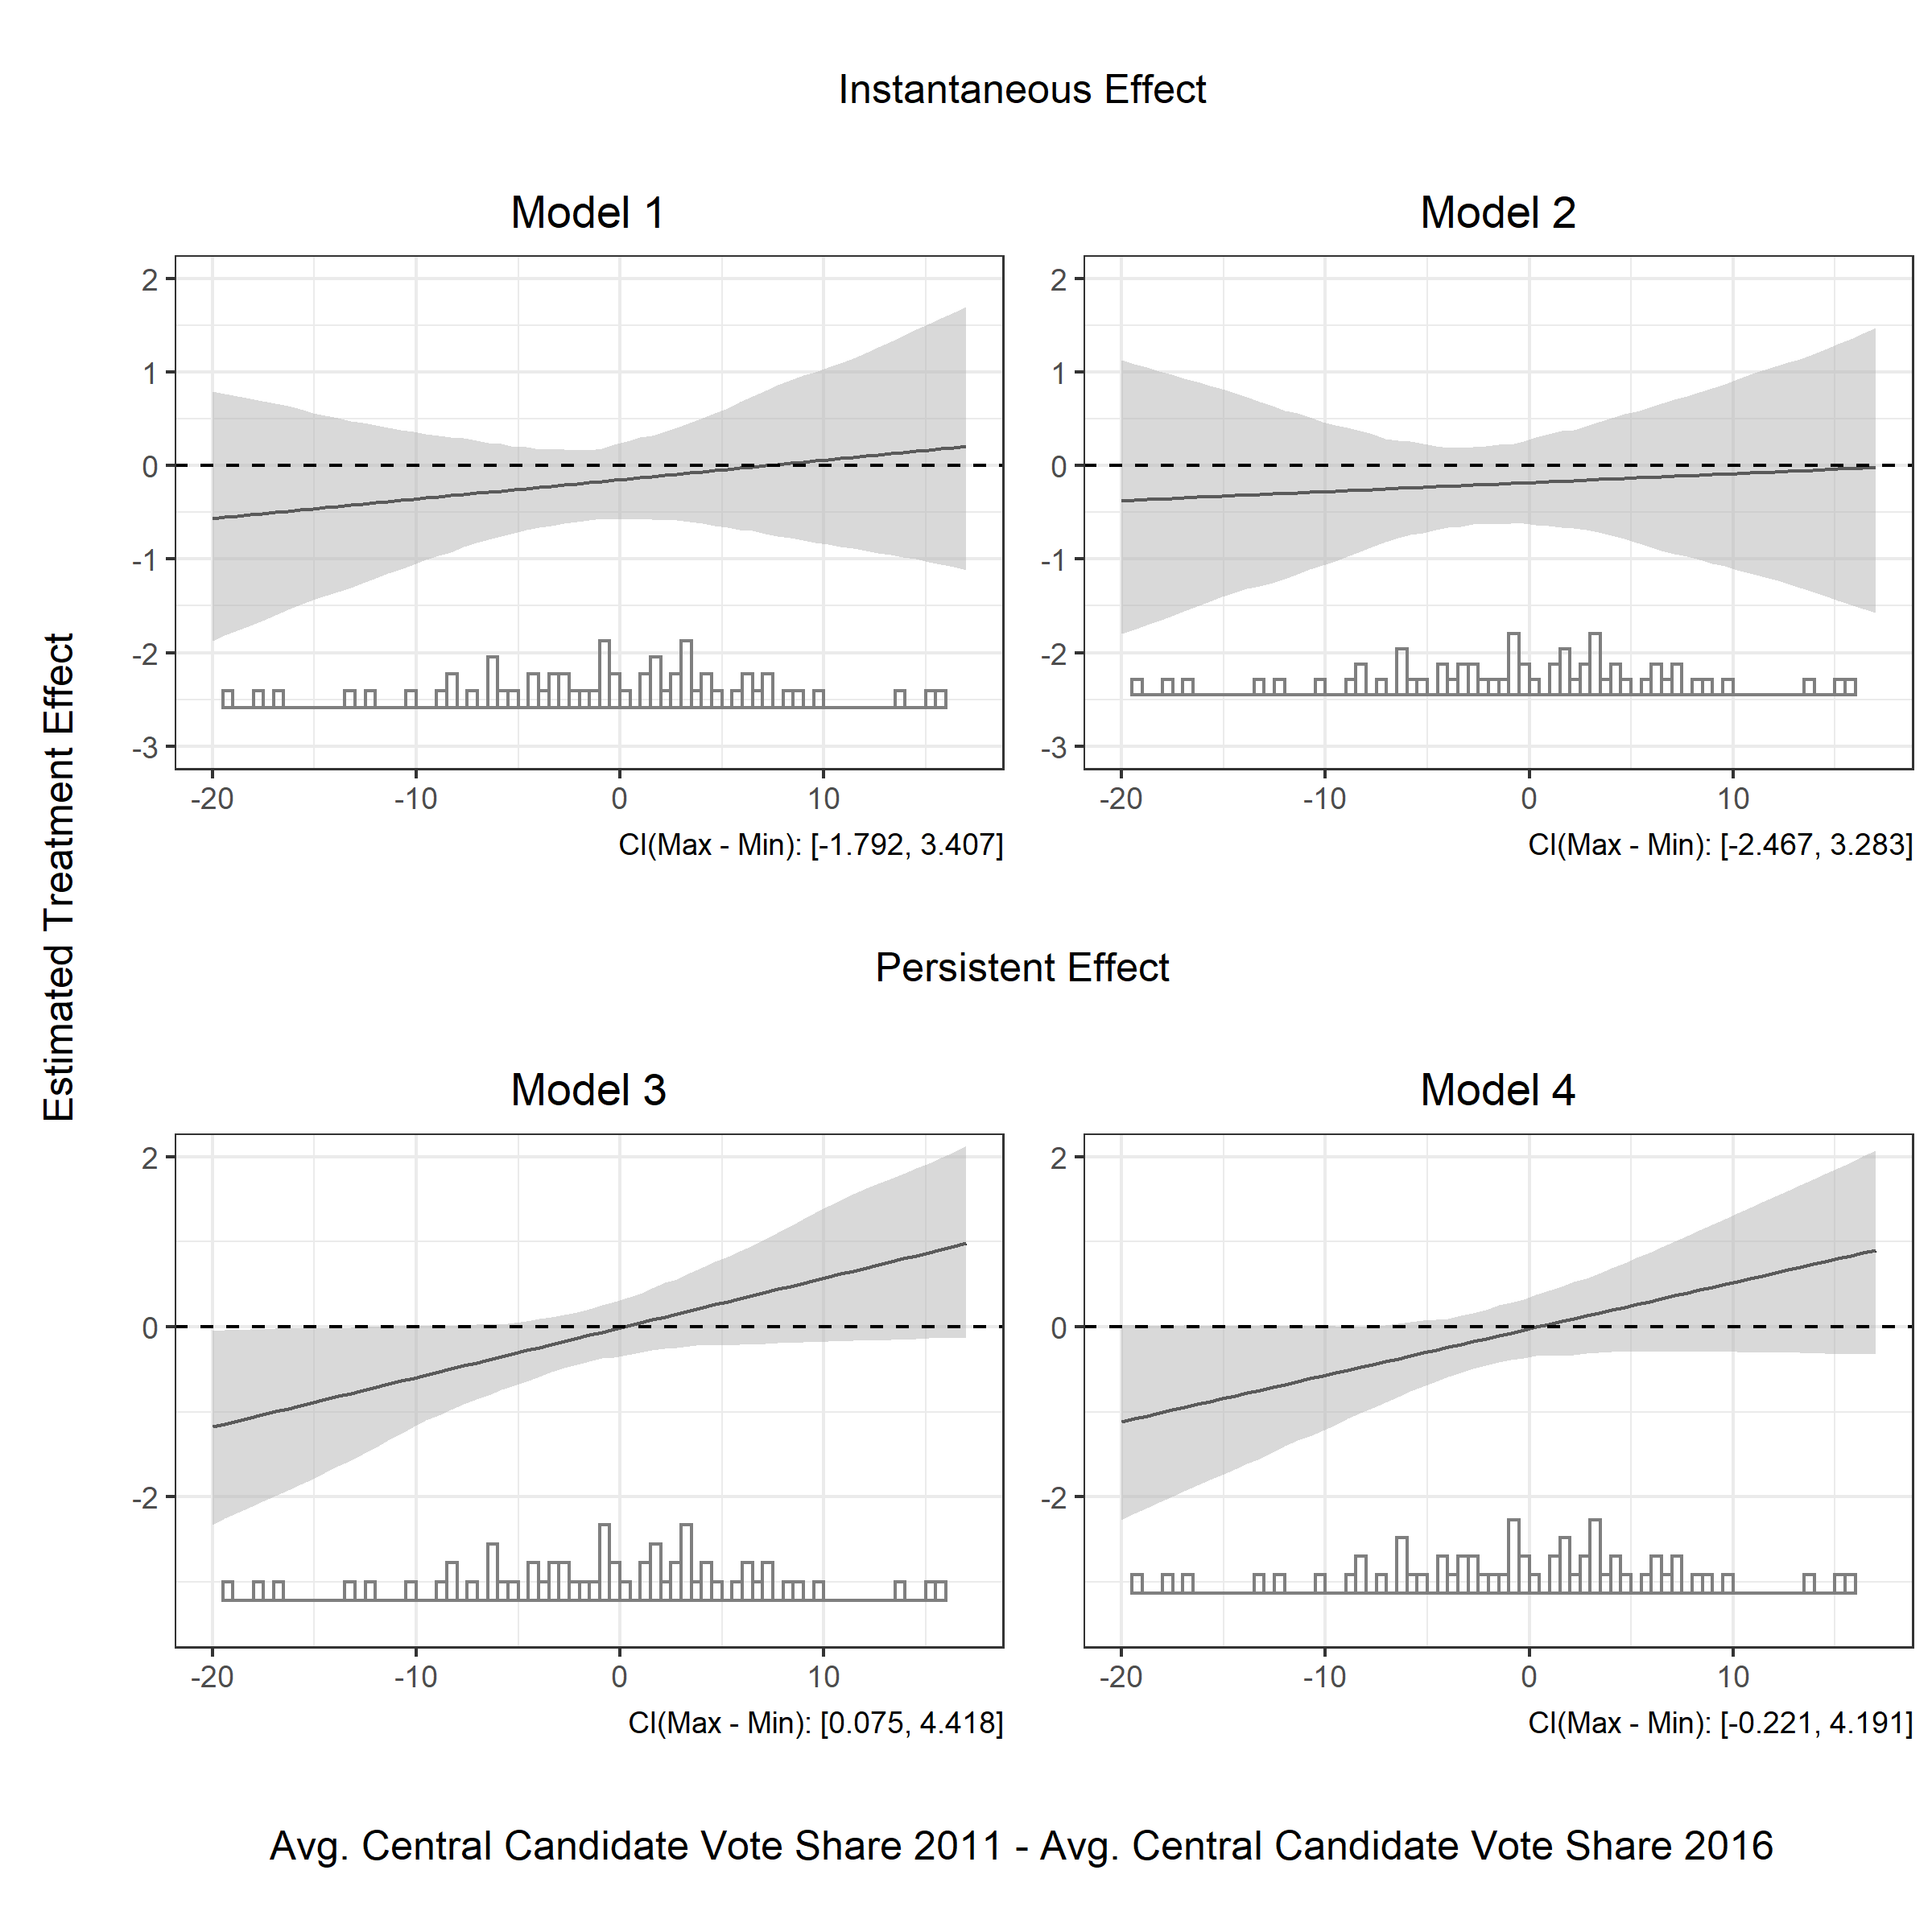
\includegraphics[width=\textwidth]{figure/200218_lfe_share.png}
%	\captionsetup{singlelinecheck=off}
%	\caption[Effect of difference in central candidate vote share]{Estimated non-linear effect of difference in province-level average central candidate vote share across different its different values. Effect estimates are derived from \autoref{tab:lfe_share}. The distributions of calculated difference is displayed as histograms.}
%	\label{fig:lfe_share}
%\end{figure}

\section{Absence of strategic behavior by voters}
\label{app:repeat}

A concern with the CPV's possible use of a placation strategy towards citizens in provinces that delivered central candidate defeats is that the increase in central transfers may incentivize voters to keep voting against these candidates in future elections. This perverse incentive would make central candidate defeats more likely to repeat, defeating the purpose of the placation.

In light of possible strategic voting, the hypothesis that the CPV would increase central transfers to provinces with central candidate defeats if they perceived these defeats as indicators for low-support areas is still plausible under two scenarios. First of all, the CPV may underestimate voters' ability to strategically cast their votes, and thus choose the placation strategy sub-optimally. This scenario is plausible considering that VNA elections happen every four to five year, meaning that the number of iterations needed for the CPV to learn about voters' strategic behaviors is small. 

The second scenario, however, is much more plausible: the CPV knows strategic voting is difficult because it demands too much from the voters. First, voters must be fully aware that delivering central candidate defeats can lead to increased funding to their provinces. However, to the best of my knowledge, this manuscript is one of the first to ever document this relationship in Vietnam. For the average voters, because elections take place only every four to five years, and then only after the national Party Congress where many other central-level decisions are also made, it is not easy to attribute any improvement in welfare to the election results specifically. Furthermore, the CPV (perhaps not coincidentally) keeps details of the budget negotiations confidential from the public, and never publicly claim credit for central transfers increases, let alone acknowledging that it increased central transfers in response to central candidate defeats in VNA elections. 

Second, strategic voting requires a sufficient numbers of voters to coordinate. For a typical electoral district with about $300,000$ voters, about $120,000$ must vote against the central candidate for this candidate to have fewer than a 60\% vote share. In addition, these voters must also agree to vote for the same set of local candidates to avoid spreading votes too thinly. Because there is no organized opposition, and because the CPV is averse to and thus would quickly suppress collective action by citizens in general, this level of coordination cannot be expected.

Finally, individual voters must find the returns from strategic voting to exceed the cost of voting against the regime's interests. My interviews suggest that, although voters do not believe their votes are traceable and can lead to direct punishment, the act of voting against regime agents' recommendation alone incurs non-trivial psychological costs, such that they only do so when feeling truly frustrated. This is consistent with the evidence by \citet{Miller2015}, who finds that perception of individual costs prevents voters from voting strategically, allowing placation strategies to remain an equilibrium in many authoritarian regimes.

For these many reasons, from the CPV's perspective, a placation strategy through central transfers increases remain the appropriate response to signals about the distribution of regime popularity coming from election results. To confirm that the CPV's discounting of strategic response is appropriate, I present evidence showing that voters were not sufficiently incentivized to keep voting against the regime following defeats in the previous election. Indeed, whereas strategic voting would have predicted election defeats to repeat once it happened, data combining multiple VNA elections confirm only the opposite.

Specifically, \autoref{tab:lfe_repeat} shows the results from three linear fixed effects models applied on province-election year data for the 2011 and 2016 elections. The model in Column 1 uses only central candidate defeat from the previous election to predict central candidate defeat in the present election. Although not statistically significant (likely due to power issue), the result shows a clear descriptive relationship: all else being equal, provinces that have experienced a central candidate defeat in a previous election is 28\% less likely to experience another defeat in the present election. 


% Table created by stargazer v.5.2.2 by Marek Hlavac, Harvard University. E-mail: hlavac at fas.harvard.edu
% Date and time: Tue, Feb 25, 2020 - 11:02:42 PM
\begin{table}[!htbp] \centering 
  \caption{Estimated effects of past central candidate defeat and net transfer changes
          on probability of defeat from linear fixed effects models} 
  \label{tab:lfe_repeat} 
\begin{tabular}{@{\extracolsep{5pt}}lccc} 
\\[-1.8ex]\hline 
\hline \\[-1.8ex] 
\\[-1.8ex] & (1) & (2) & (3)\\ 
\hline \\[-1.8ex] 
 Previous Central Candidate Defeat & $-$0.284 & $-$0.292 & $-$0.340 \\ 
  & (0.241) & (0.219) & (0.239) \\ 
  (Logged) Net Transfer Change &  & 0.008 & 0.006 \\ 
  &  & (0.005) & (0.005) \\ 
  Previous Central Candidate Defeat $\times$ \\ (Logged) Net Transfer Change &  &  & 0.011 \\ 
  &  &  & (0.017) \\ 
 \hline \\[-1.8ex] 
Province FEs & Yes & Yes & Yes \\ 
Year FEs & Yes & Yes & Yes \\ 
\hline \\[-1.8ex] 
N & 120 & 120 & 120 \\ 
R$^{2}$ & 0.779 & 0.807 & 0.818 \\ 
\hline 
\hline \\[-1.8ex] 
\multicolumn{4}{l}{$^{*}$p $<$ .1; $^{**}$p $<$ .05; $^{***}$p $<$ .01} \\ 
\end{tabular} 
\end{table} 


Furthermore, in Column 2, I add to the model the log of changes in net transfers from the previous election, which is the outcome variable in the main analysis but measured for the previous election. The coefficient is small and indistinguishable from zero, suggesting that changes in net transfers following the previous election has no clear impact on the present election, once the tendency of election defeats to \textit{not} repeat has been accounted for. 

In Column 3, I add an interaction term between the two variables; this interaction term would help identify whether changes in net transfers have any particular effect in provinces that have experienced central candidate defeats in the previous election. This conditional effect, obtained by summing the second and third coefficients in Column 3, remains small and indistinguishable from zero. Specifically, the conditional effect estimate is $.017$ and has a 95\% confidence interval of $[-.014,.048]$. The point estimate alone indicates that an increase in net transfers that is equivalent to 1\% of the year-to-year average change would increase the probability of central candidate defeats by 1.7\%, equivalent to $1/20$ of the first coefficient. In other words, provinces that experience central candidate defeats in one election would \textit{not} be more likely to see a repeated defeat unless its net transfers were increased by 20\% of the year-to-year average change. In contrast, the effect estimated in the main manuscript translates to only an 9.1\% increase.

Overall, even though the independent variables in these models are far from exogenous and thus do not allow for strong causal claims, this analysis provides ample descriptive statistics to suggest that the CPV's placation strategy is sustainable. Specifically, even after accounting for the increases in central transfers, provinces that witnessed central candidate defeats in one election are still less likely to experience a repeated defeat.

\clearpage
\inputencoding{utf8}
\printbibliography[heading=bibintoc]


\end{document}


